\chapter{Data Reduction and Analysis}
	\label{cha:Data}
This chapter presents our observations of the Southern Sample (as laid out in Section \ref{sec:Sample}) made with the Visible Multi-object Spectrograph (VIMOS; see Section \ref{sec:VIMOS}) on the European Southern Observatory's (ESO's) Very Large Telescope (VLT). The data-reduction pipeline is described in Section \ref{subsec:VIMOSreduction} along with a discussion of the data quality and the artefacts caused by VIMOS data in Section \ref{subsec:VIMOSartefacts}. A brief discussion of alternative data-reduction pipelines for VIMOS data is given in Section \ref{subsec:Other}. Unpublished archival observations made with the VLT's Multi-unit Spectroscopic Explorer (MUSE) are also used in this project and are described in Section \ref{sec:MUSE}, along with a discussion of ESO's data-reduction pipeline in Section \ref{subsec:MUSEreduction}. Finally, in Section \ref{sec:analysis}, we describe our own data-analysis pipelines, that are used to produce the results presented in Chapters \ref{cha:stellar} and \ref{cha:gas}. 

\section[The Visible Multi-object Spectrograph (VIMOS)]{The Visible Multi-object Spectrograph \\(VIMOS)}
	\label{sec:VIMOS}
	\subsection{VIMOS Instrument}
		VIMOS is a fibre-fed, multi-purpose spectrograph mounted on Unit Telescope 3 (UT3) of ESO's VLT in Paranal, Chile \citep{LeFevre2003}. It has a number of configurations: direct imaging, multi-object spectroscopy (MOS) or integral-field spectroscopy (IFS). For our program, VIMOS was used in IFS mode. 

		The integral-field unit (IFU) has a field of view of $40 \times 40$ spatial pixels (spaxels) with a focal elongator at the entrance to the IFU offering choice of spatial sampling of $0 \farcs67$ or $0 \farcs33$ per spaxel. There are 6 available grisms with varying wavelength ranges and spectral resolutions: low- and high-resolution (LR or HR) red; HR orange; and LR, medium resolution (MR) and HR blue. The observations presented in the following section were obtained using the new (as of March 2012 with our observations obtained in April--November 2012; see Table \ref{tab:observations}) HR blue grism with a spatial sampling of $0 \farcs67$ per spaxel. 

		\begin{figure}
			\centering
			
\includegraphics[width=0.4\textwidth]{chapter2/quadrants.png}
			\caption[Schematic of the VIMOS quadrants]{A Schematic of the VIMOS quadrants.}
			\label{fig:quadrants}
		\end{figure}

		The field of view of VIMOS is split into 4 quadrants (cheerfully named in the Flexible Image Transport System, FITS, headers, Brian, Keith, Tom and David). A schematic of the layout is shown in Fig.\,\ref{fig:quadrants}. The quadrants are operated in parallel as independent detectors and it is not possible to use different grisms with different quadrants. The IFU fibres are arranged in a row parallel to and above the short sides of the charge-coupling device (CCD) detectors, and the light from each fibre is then dispersed by the grism in the other direction. This gives rise the to row-stack spectra (RSS) format of most fibre-fed IFU devices.

		VIMOS has several well-known though poorly-understood technical issues. These include several low transmission (bad) fibres, strong flexure and large differences in sensitivity across its 4 quadrants. These are partially dealt with using a specialist data-reduction pipeline described in Section \ref{subsec:VIMOSreduction}, with a discussion of the resulting data quality presented in Section \ref{subsec:VIMOSartefacts} (for more details see the instrument manual, Section 2.8 in the version for Observing Period 100\footnote{\url{http://www.eso.org/sci/facilities/paranal/instruments/vimos/doc.html}}).

	\subsection{VIMOS Observations}
		As stated above, observations for our project were obtained using the VIMOS IFS mode with a spatial sampling of $0\farcs67$ per spaxel and the HR blue grism, yielding a wavelength range of 3700-5520\,\AA\ with a spectral resolution of 1440 and sampling of 0.71\,\AA\,$\mathrm{pix^{-1}}$. Our program (ID: 089.B-0632A) ran in service mode during ESO's period 89 and 90. Each object was observed with a total integration time of $\approx 100$\,min on-source, equally spread over three observing blocks (OBs). Each OB contained 2 science exposures followed by 3 continuum lamp exposures for flatfielding and finally 1 He-Ne arc lamp exposure for wavelength calibration. In addition, the standard VIMOS calibration programme provided 5 bias exposures per night. The flux calibration was calculated using publicly available observations of the spectro-photometric standard star Feige 110 provided by ESO. A summary of the observations is given in Table \ref{tab:observations}.


		\begin{table}
			\centering
		\begin{threeparttable}
			\caption{A summary of the VIMOS observational logs.}
			\label{tab:observations} 
			\begin{tabular}{c c c c c c c}
			\hline
			\hline
				Galaxy 	& OB & Date & Av. DIMM & I. seeing & F. seeing & Airmass \\
				& & (2012) & (arcsec) & (arcsec) & (arcsec) & (arcsec) \\
			\hline
				\multirow{3}{*}{ESO 443-G24}& 1 & 15 Apr & 0.79 & 0.83 & 0.71 & 1.023 \\
				& 2 & 27 Apr & 2.14 & 2.67 & 1.69 & 1.012 \\
				& 3 & 27 Apr & 2.36 & --\tnote{a} & 2.78 & 1.039 \\
			\hline
				\multirow{3}{*}{IC 1459}& 1 & 21 May & 0.82 & 0.84 & 0.82 & 1.238 \\
				& 2 & 28 May & 1.20 & 1.26 & 1.01 & 1.175 \\
				& 3 & 18 Jun & 1.10 & 1.27 & 1.09 & 1.277 \\
			\hline
				\multirow{3}{*}{IC 1531}& 1 & 18 Jun & 1.12 & 1.45 & 1.07 & 1.292 \\
				& 2 & 18 Jun & 1.21 & 1.29 & 1.38 & 1.137 \\
				& 3 & 16 Jul & 1.05 & 1.03 & 0.98 & 1.149 \\
			\hline
				\multirow{3}{*}{IC 4296}& 1 & 23 Apr & 0.78 & 1.00 & 0.61 & 1.015 \\
				& 2 & 23 Apr & 1.09 & 0.90 & 0.86 & 1.101 \\
				& 3 & 23 Apr & 0.86 & 1.07 & 0.89 & 1.224 \\
			\hline
				\multirow{3}{*}{NGC 612}& 1 & 25 Jun & 0.74 & 0.72 & 0.78 & 1.244 \\
				& 2 & 19 Jul & 1.25 & 1.45 & 1.46 & 1.177 \\
				& 3 & 19 Jul & 1.19 & 1.08 & 1.11 & 1.076 \\
			\hline
				\multirow{3}{*}{NGC 1399}& 1 & 27 Jul & 1.09 & 0.95 & 1.28 & 1.314 \\
				& 2 & 29 Jul & 1.02 & 0.95 & 1.04 & 1.219 \\
				& 3 & 15 Aug & 1.51 & 1.06 & 1.57 & 1.281 \\
			\hline
				\multirow{3}{*}{NGC 3100}& 1 & 15 Apr & 0.76 & 0.76 & 0.82 & 1.017 \\
				& 2 & 15 Apr & 0.79 & 0.75 & 0.82 & 1.066 \\
				& 3 & 25 Apr & 1.22 & 1.16 & 1.20 & 1.010 \\
			\hline
				\multirow{3}{*}{NGC 3557}& 1 & 27 Apr & 0.89 & 1.08 & 0.71 & 1.033 \\
				& 2 & 27 Apr & 1.10 & 0.80 & 0.96 & 1.030 \\
				& 3 & 27 Apr & 1.66 & 1.46 & 1.36 & 1.065 \\
			\hline
				\multirow{3}{*}{NGC 7075}& 1 & 18 May & 1.29 & 1.64 & 1.02 & 1.138 \\
				& 2 & 19 May & 0.91 & 1.18 & 0.66 & 1.200 \\
				& 3 & 21 May & 0.87 & 0.80 & 1.33 & 1.229 \\
			\hline
				\multirow{3}{*}{PKS 718-34}& 1 & 15 Apr & 1.02 & 0.99 & 0.95 & 1.113 \\
				& 2 & 16 Apr & 1.05 & 1.25\tnote{b} & 1.05 & 1.126 \\
				& 3 & 12 Nov & 0.69 & 0.68 & 0.65 & 1.146 \\
			\hline
			\hline
		\end{tabular}
			\begin{tablenotes}
			\footnotesize
			\note Col.\,1: Galaxy name. Col.\,2: Observation block (OB) number. Col.\,3: Date of observation. Col.\,4: Average differential image motion monitor(DIMM) during OB. Col.\,5: Initial seeing. Col\,6: Final seeing. Col\.7: Average airmass during OB.
			\item [a] Failed seeing reading at both start and end of first exposure for ESO 443-G24, OB 3 
			\item [b] Failed seeing reading at start of first exposure for PKS 718-34, OB 2. Seeing from end of exposure quoted instead. 
			\end{tablenotes}
		\end{threeparttable}
		\end{table}

	\subsection{VIMOS Data Reduction}
		\label{subsec:VIMOSreduction}
		The data-reduction pipeline we adopted was produced using \textsc{Py3D}, a suite of programs based on the \textsc{python} versions of those developed for the Calar Alto Legacy Integral Field spectroscopy Area survey \citep[CALIFA;][]{Sanchez2012, Husemann2013} but later updated for VIMOS by \citet{Husemann2014}. \textsc{Py3D} was provided to us by Husemann and is not currently publicly available. It makes use of pixel tables to track each pixel throughout the pipeline, with both spectral and spatial resampling only occurring once. The pipeline attempts to account for many of the known issues with VIMOS, such as bad fibres, strong flexure and contamination from adjacent spectra on the CCD (cross-talk), in addition to standard reduction procedures for IFS data. A full outline of the reduction is given below.

		A median `master' bias is first created from the five daily bias frames and subtracted from each raw frame. Known low-transmission (bad) fibres, identified cosmic rays and offsets accounting for flexure of the instrument due to gravity are all considered when automatically identifying the fibre peak positions on the detector. Each fibre is then traced along the dispersion axis in the flat frames. \citet{Husemann2014} find this process to be robust, except for a few fibres at the very blue end of the spectra ($<4300$\,\AA). 

		Since flexure is dependent on the altitude of the pointing of the telescope and the rotation of the instrument, the science exposures will be affected in a manner slightly different than the flatfield exposures. \textsc{Py3D} accounts for these offsets by tracing the peak of the cross-dispersion profile directly on the science exposures at 5 or 6 locations along the dispersion direction for each spectra. The offsets between these positions and the traced spectra at the relevant wavelengths in the flatfield exposures are then interpolated along the dispersion axis with a second order Legendre polynomial. This procedure corrects for the flexure in the cross-dispersion direction, but flexure also affects the dispersion direction due to differences in the pointing of the telescope between the science and arc lamp exposures. This effect is estimated by measuring the positions of strong sky emission lines, but our HR blue grism data have only one sky line at 5199\,\AA, which in many of our science frames was very dim or not detected. This lack of sky lines had previously been an issue with our initial attempt at data reduction using the publicly available \textsc{p3d} suite of programs\footnote{\url{http://p3d.sourceforge.net/}}. Here the lack of sky lines means that \textsc{p3d} is not able to flux calibrate the quadrants with respect to each other. For this reason (and the lack of flexure correction), we use \textsc{Py3D} instead.

		Another issue taken into account by \textsc{Py3D} is cross-talk, where fibres are so densely packed that light from one fibre contaminates (in the cross-dispersion direction) that of neighbouring fibres. The spectra are extracted assuming a Gaussian profile for each fibre in the cross-dispersion direction, with the Gaussian width fitted for each fibre individually. After this, the spectra are adaptively smoothed to a 3\,\AA\ full-width at half-maximum (FWHM) resolution in the dispersion direction and are resampled to a common wavelength solution.

		Flatfields are used to correct for the different transmission efficiencies of the fibres and the different sensitivities of the CCD pixels. Observations of the spectro-photometric standard star Feige 110, recorded in each of the 4 quadrants, are obtained automatically by ESO and are reduced in the same way as described above. Comparisons of the resulting spectra to a reference spectrum of Feige 110 provided by Husemann (private communication) are then used to flux calibrate each quadrant. For each quadrant in every science frame a mean sky spectrum is built using spectra from the outer regions of the field of view and subtracted.

		The quadrants are then combined into a single file, converted from the RSS format to a standard cube (with dimensions of right ascension, declination and wavelength $\lambda$). Finally, the change of the position of the centre of the galaxy with wavelength (due to differential atmospheric refection, DAR) is measured and corrected for. 

		% created with VIMOS_project/reduction/show_corrections.py
		\begin{figure}
			\centering
			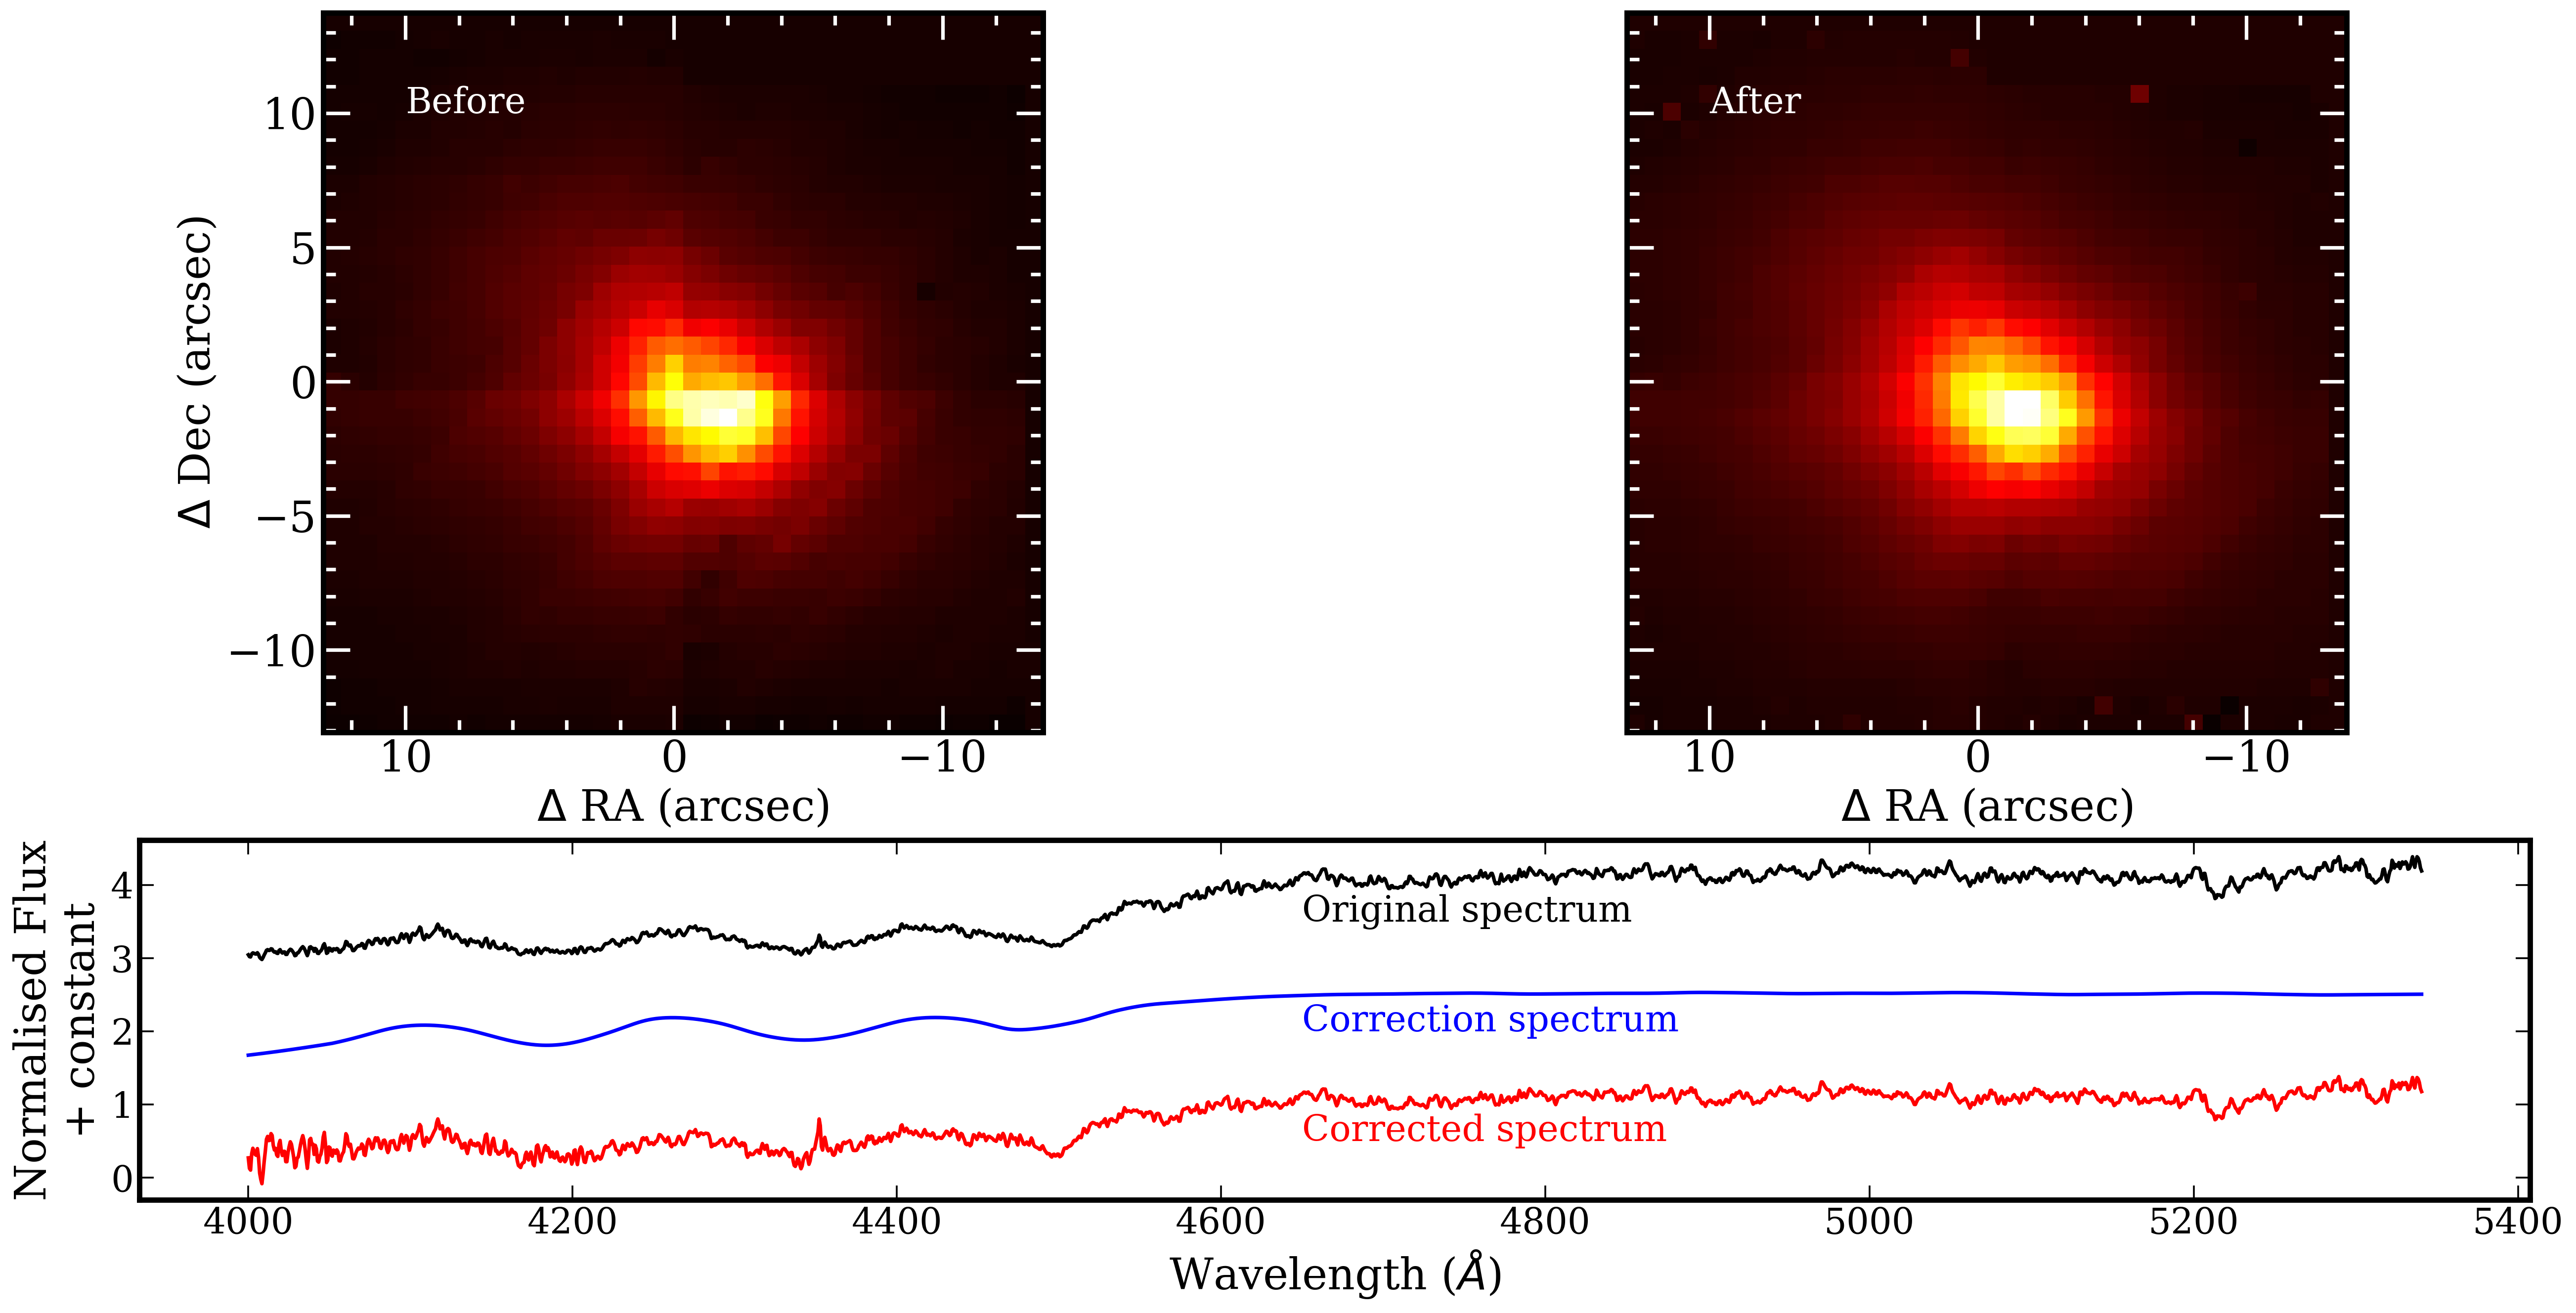
\includegraphics[width=0.99\textwidth]{chapter2/corr_image.png}
			\caption[Ad-hoc correction to the VIMOS datacubes]{Effects of the ad-hoc corrections applied as part of the VIMOS data-reduction pipeline. The top panels show the reconstructed image before (left) and after (right) the ad-hoc corrections are applied to the NGC 3557 datacube. The corrections aim to improve the quadrant-to-quadrant calibration and reduce diagonal intensity stripes. The bottom panel shows an example of the fringe-like pattern correction applied to a single spaxel in NGC 3100.}
			\label{fig:Correction}
		\end{figure}

		Following this, we noted that the cubes were still not properly calibrated. Three main issues remain: the quadrants have different intensities, clearly showing uncorrected throughput differences; diagonal intensity stripes are present in the reconstructed images at all wavelengths; and spectral features are observed \citep{Jullo2008} that are visually similar to fringe patterns caused by interference within the CCD between incident light and light reflected from the interfaces between layers of the CCD materials. Given the thickness of the CCD layers, such fringes should only be observed at $>7000$\,\AA, however they can be seen at all wavelengths, suggesting a different origin. \citet{Lagerholm2012} notes that they appear to be due to altitude angle and hysteresis-dependent reflections occurring within the fibres. We refer to these features hereafter as fringe-like patterns. The first two of these issues are illustrated in the top-left panel of Fig.\,\ref{fig:Correction}. \citet{Lagerholm2012} pointed out that the intensity stripes do not seem to be bound by the quadrants, and concluded that they therefore probably originate from an unknown data-reduction pipeline problem. They however made use of the data-reduction pipeline supplied by ESO\footnote{\url{http://www.eso.org/sci/software/pipelines/vimos/}}, while we use \textsc{Py3D} and also observe the intensity stripes, suggesting that the specific pipeline may not be the cause. 

		These issues were corrected by implementing a \textsc{python} version of the ad-hoc corrections given in \citet{Lagerholm2012}. This involves re-normalizing the quadrants to each other by finding the multiplicative factor for each quadrant which minimizes the differences of the integrated spectra of neighbouring fibres across the edges of neighbouring quadrants (quadrant 2 is held constant). This is followed by the removal of the fringe-like pattern by constructing a correction spectrum by dividing the spectrum of a given fibre by the median spectrum from the eight fibres spatially surrounding it and smoothing over a scale of 150 pixels in the dispersion direction. Each spectrum of the original datacube is then divided by the corresponding correction spectrum (example shown for a single spaxel in NGC 3100 in the bottom panel of Fig.\,\ref{fig:Correction}). The diagonal stripes are not addressed, however the top two panels of Fig.\,\ref{fig:Correction}, which show the reconstructed images (where the datacube is collapsed in the spectral direction) of NGC 3557 before and after these corrections are applied, shows that their impact is significantly lessened by these corrections. This suggests that they may have some connection to the fringe-like patterns. 

		These additional steps mean that the datacubes are not perfectly flux-calibrated, but all the corrections are multiplicative and thus will not effect equivalent width measurements. From comparisons to the MUSE data (see Section \ref{sec:MUSE}), we can then estimate the flux calibration of the resulting datacubes. 

		The variance spectra are propagated throughout the data-reduction pipeline (including these ad-hoc corrections) and are square-rooted at this point, to be used as noise inputs in the following analyses (see Section \ref{sec:analysis}).

	\subsection{VIMOS Data Quality}
		\label{subsec:VIMOSartefacts}
		By comparing the top panels of Fig.\,\ref{fig:Correction}, we can clearly see that while there is an obvious improvement of the calibration between the quadrants, there are still sharp offsets. This often gives rise to diamond-shaped rather than elliptical isophotes. Neighbouring spaxels along the quadrant edges can have fluxes that are different by as much as 20-30\%. Luckily, the worst affected galaxies are IC 4296 and NGC 1399, for which MUSE archival data are available (see Section \ref{sec:MUSE}). 

		Similar offsets are also observed in the spectral direction, with a slight offset of the absolute wavelength calibration between quadrants. This is most clearly seen in the mean velocity maps after the routines described in Section \ref{subsec:StellarFit} are applied. For example the left panel of Fig.\,\ref{fig:egVel} shows the mean stellar velocity map of NGC 1399. The top-right quadrant clearly has a slightly higher velocity than would be expected for a normal rotating galaxy. This corresponds to a shift of the galaxy spectra with respect to the reference wavelength frame (i.e.\ the arcs lamp lines). For comparison, the right panel of Fig.\,\ref{fig:egVel} shows the mean stellar velocity map of the same galaxy from a different instrument, that does not suffer from this problem. Again, the worst affected galaxies are IC 4296 and NGC 1399.

		\begin{figure}
			\centering
			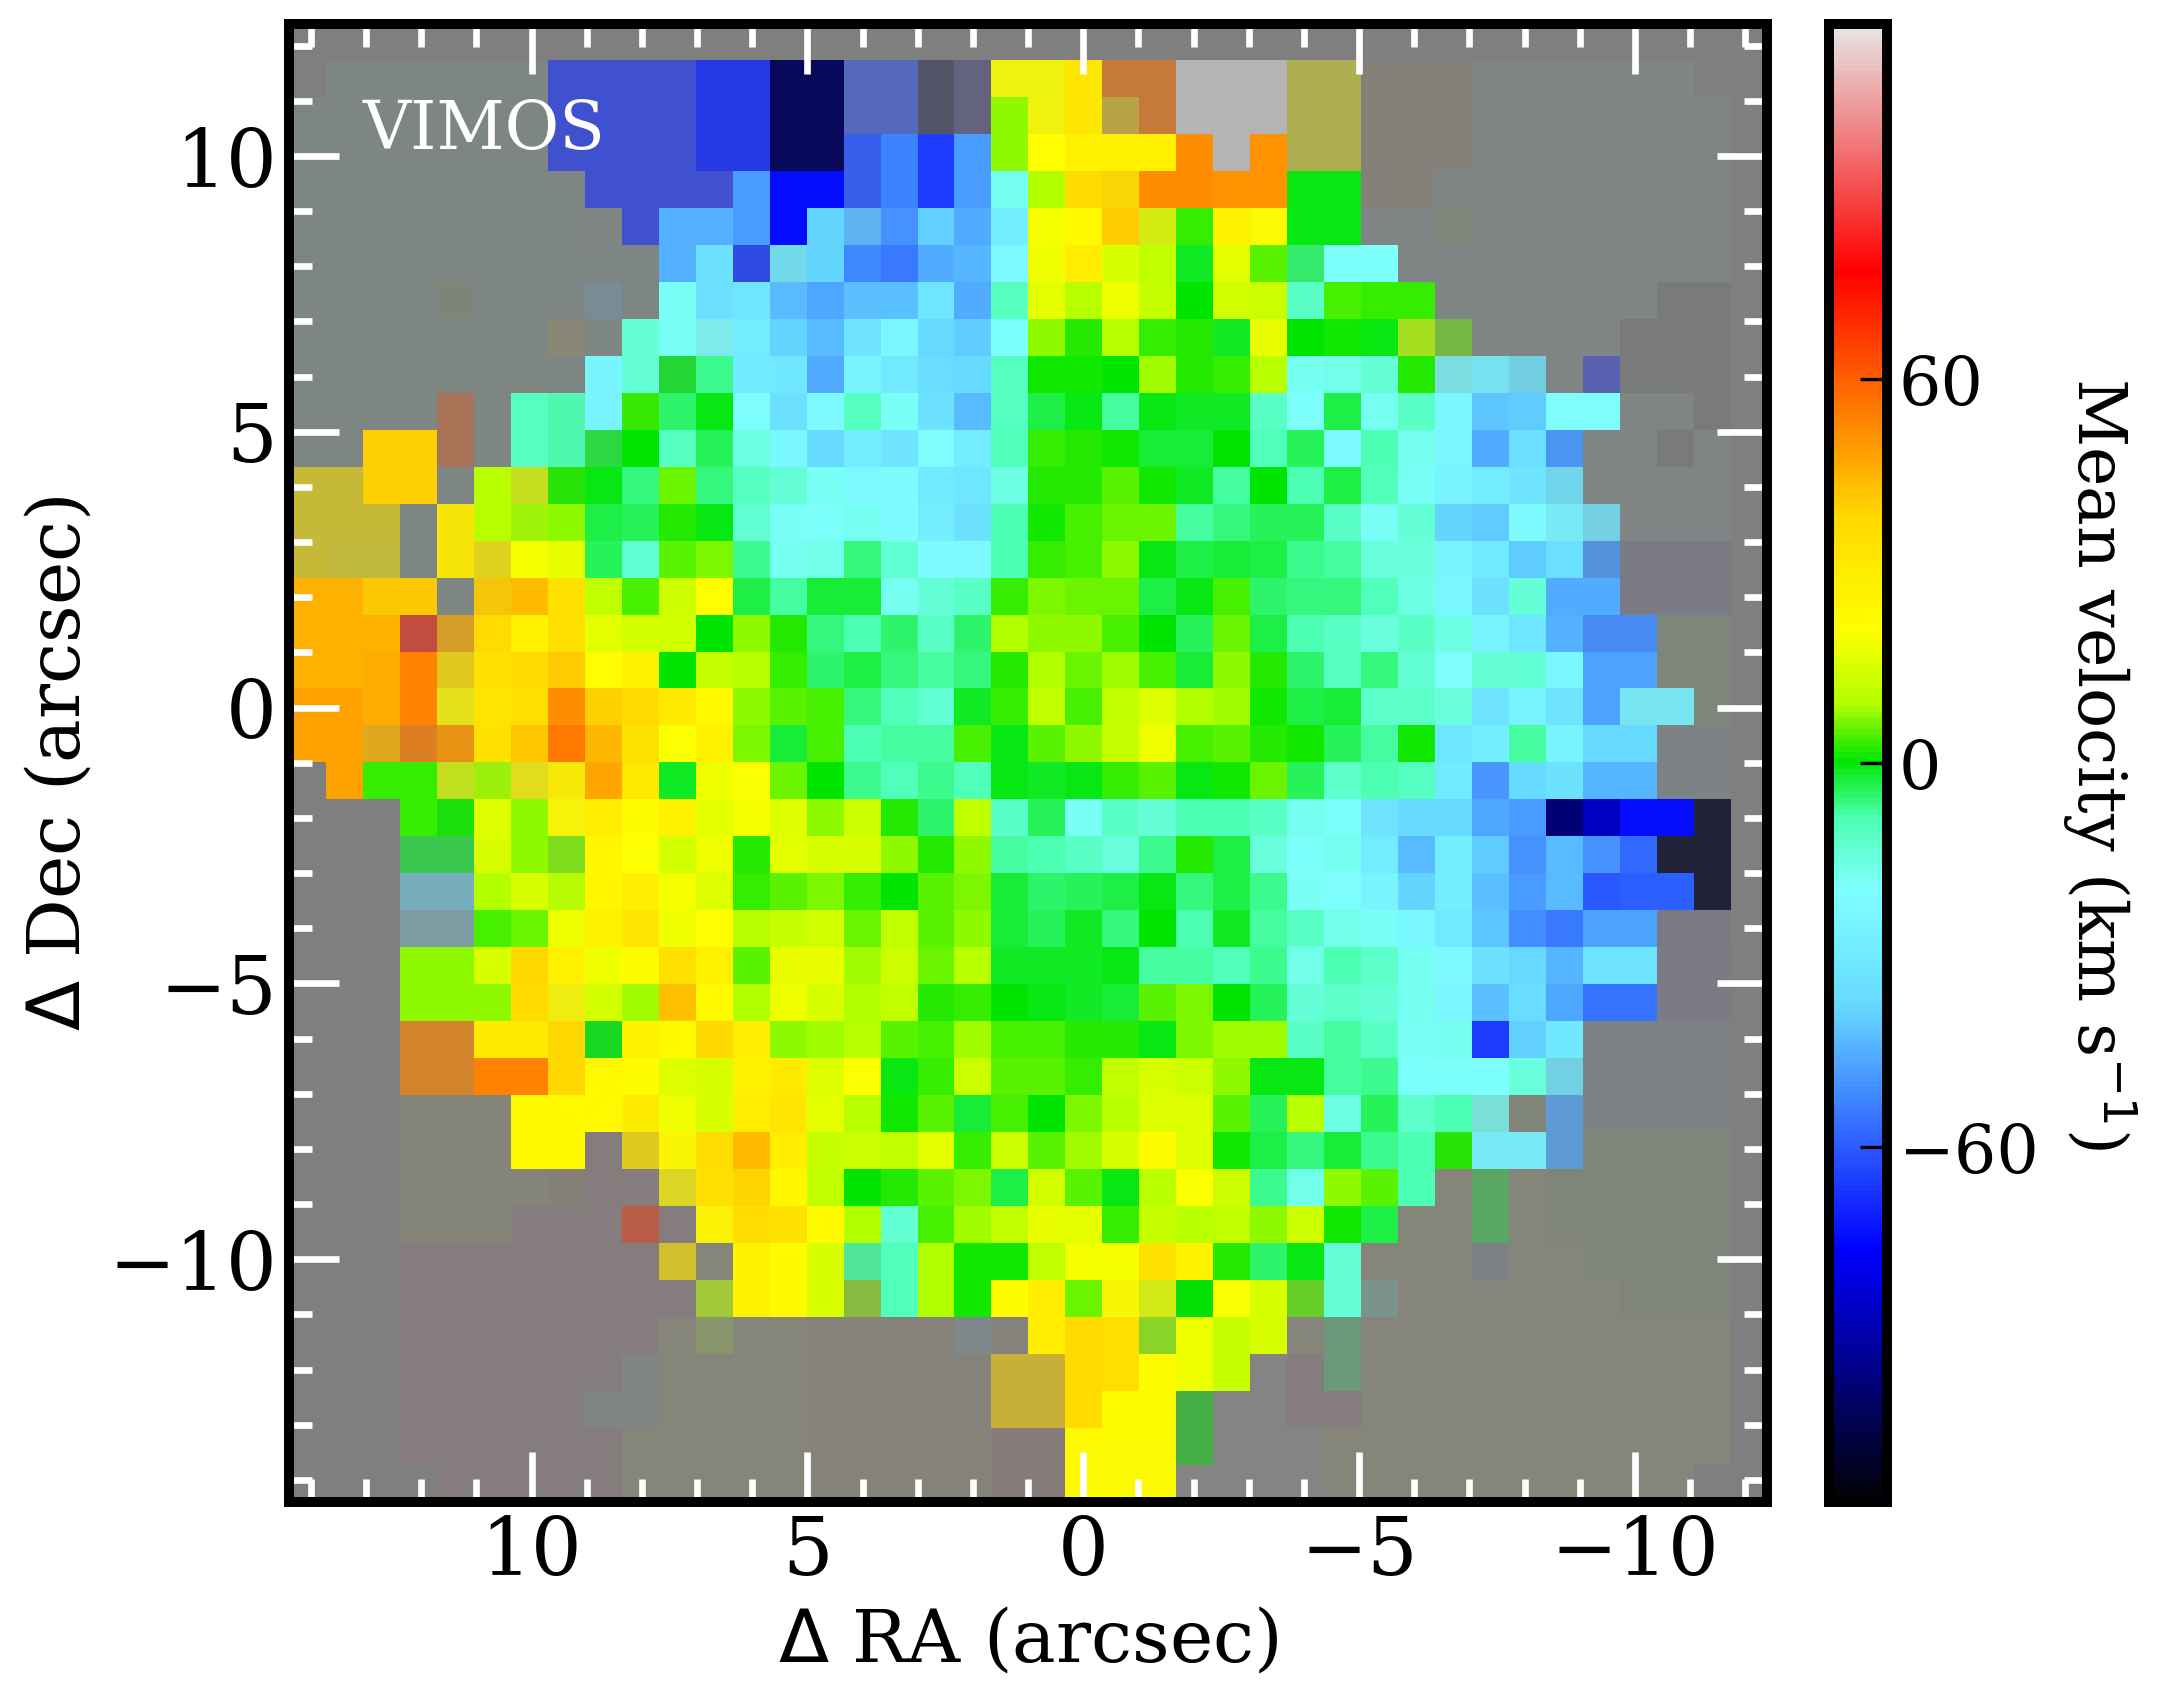
\includegraphics[width=.4\textwidth]{chapter2/VIMOS_NGC1399_vel.png}
			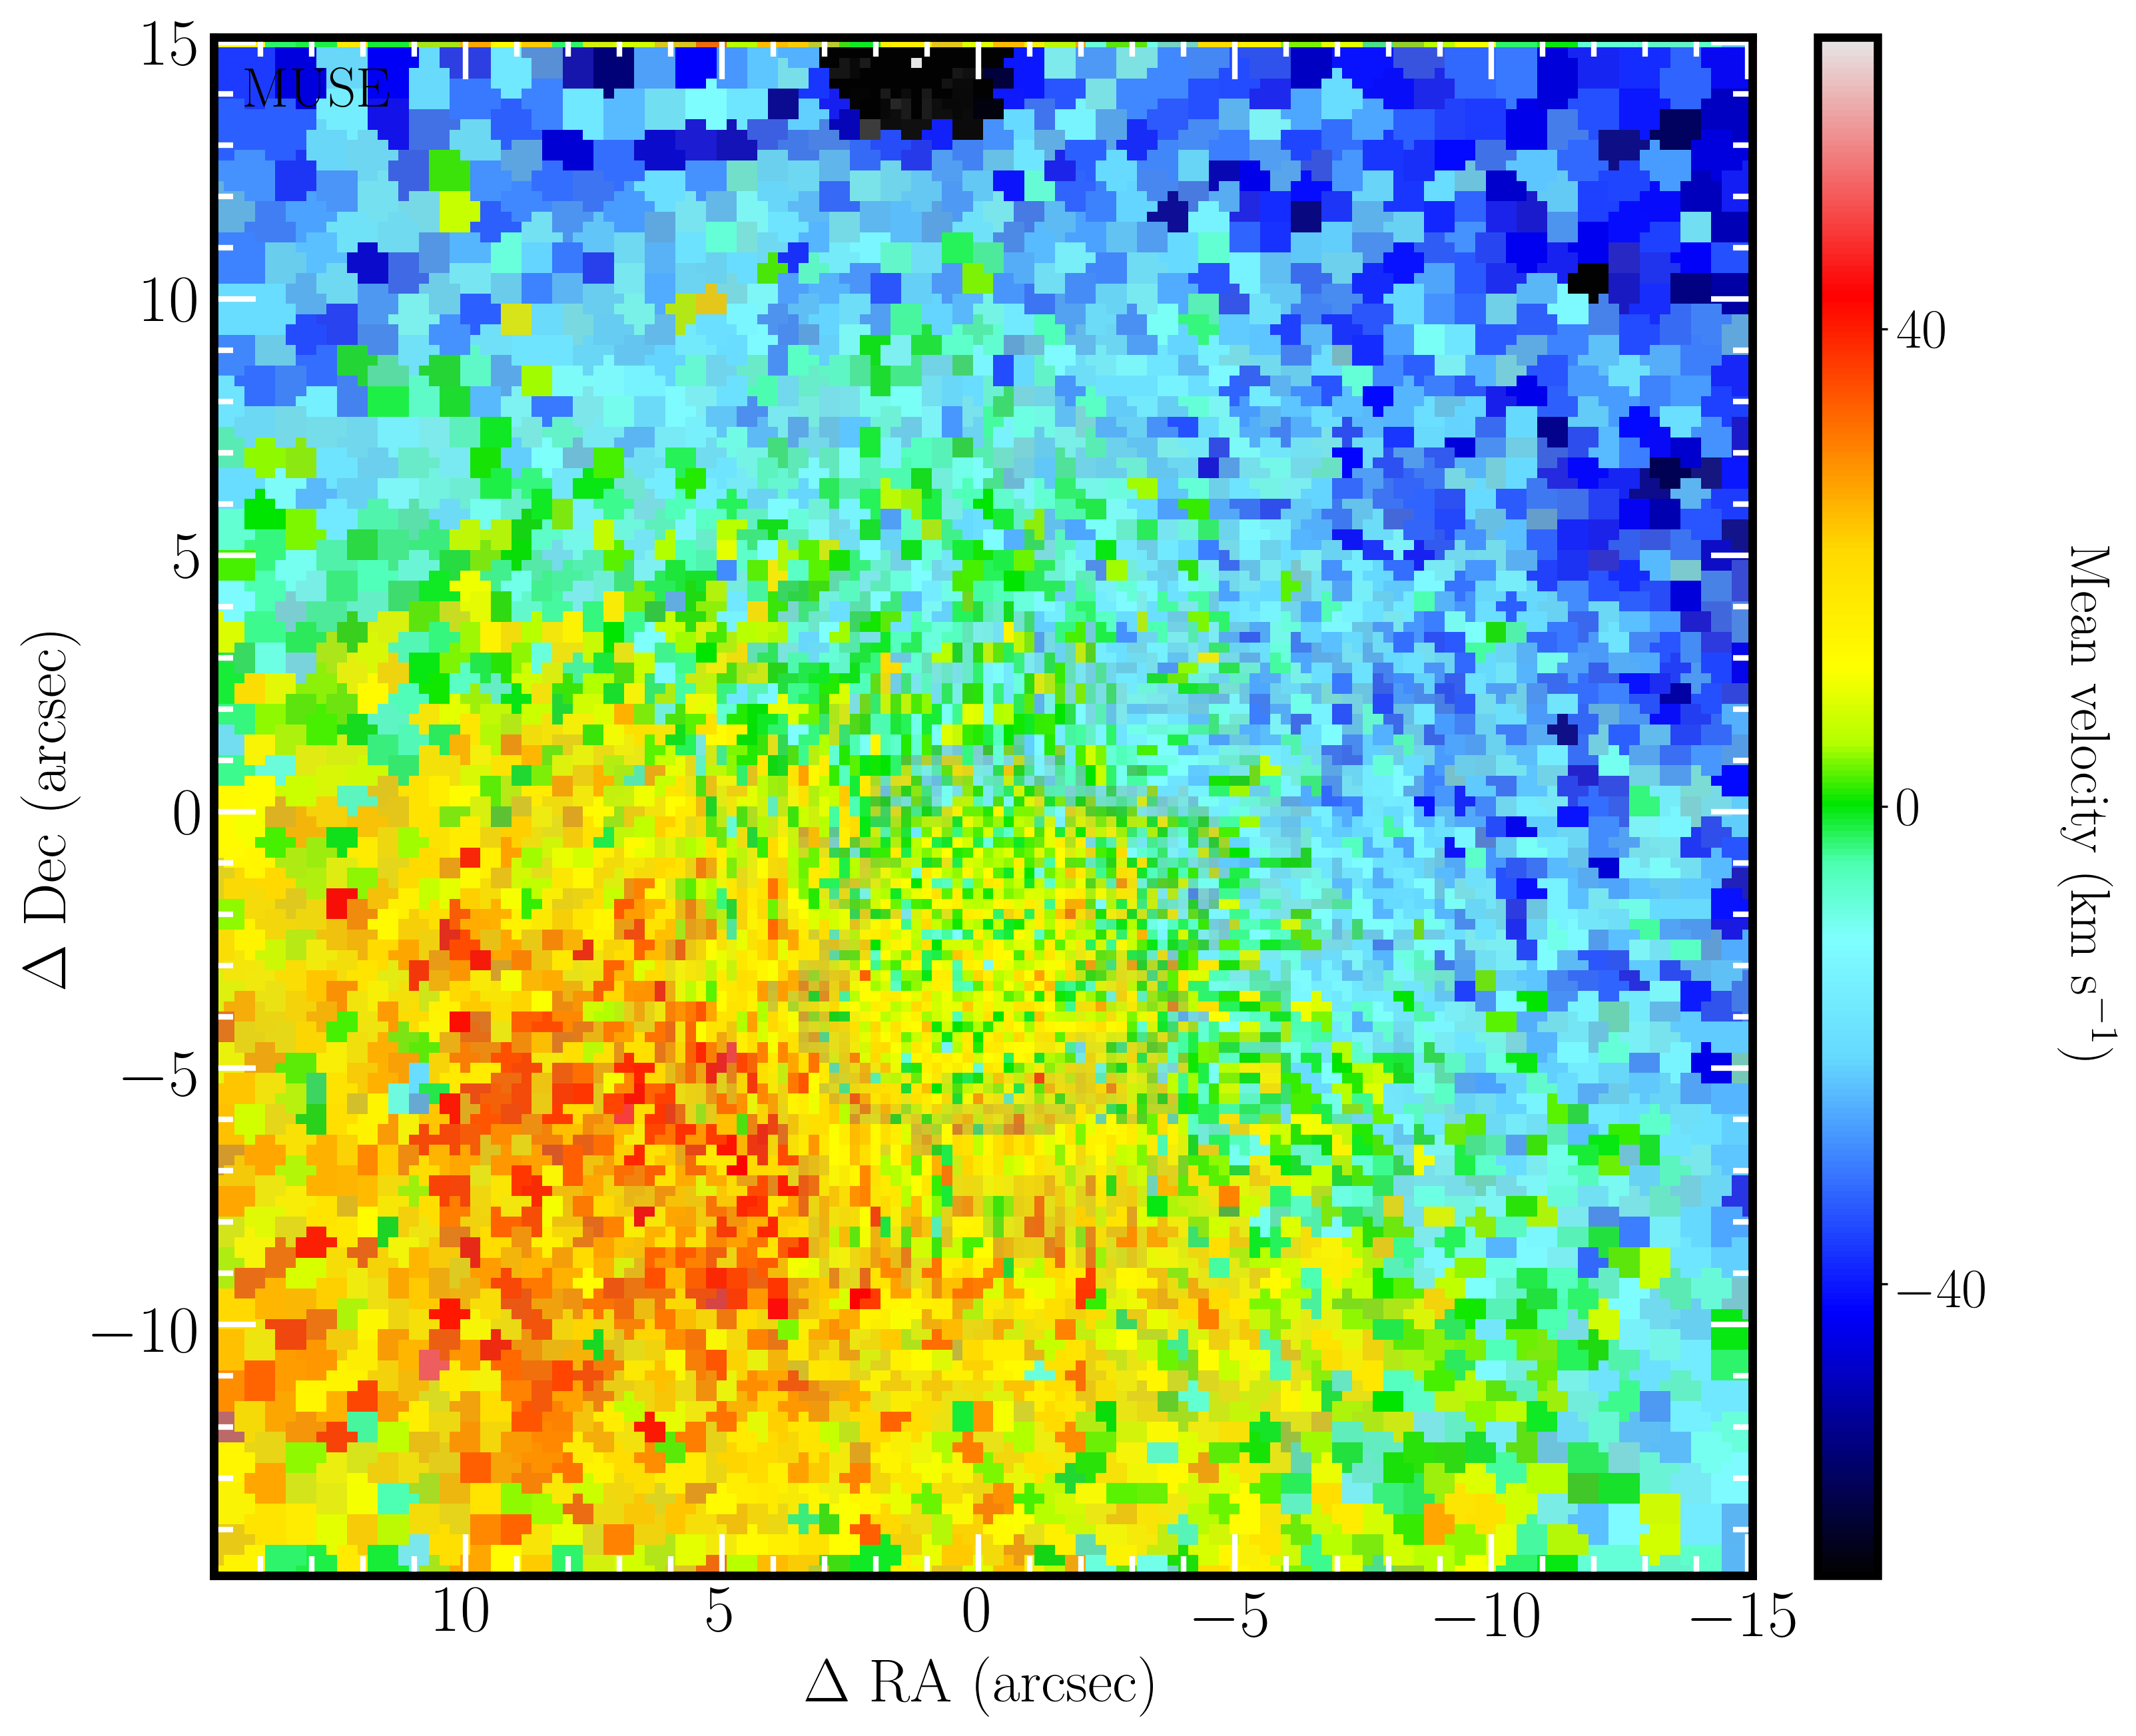
\includegraphics[width=.4\textwidth]{chapter2/MUSE_NGC1399_vel.png}
			\caption[VIMOS data wavelength calibration problems]{Mean stellar velocity maps of NGC 1399, demonstrating the wavelength calibration offsets between the different quadrants of VIMOS. Left panel: VIMOS map. Right panel: MUSE map (see Section \ref{sec:MUSE}).}
			\label{fig:egVel}
		\end{figure}

		\begin{figure}
			\centering
			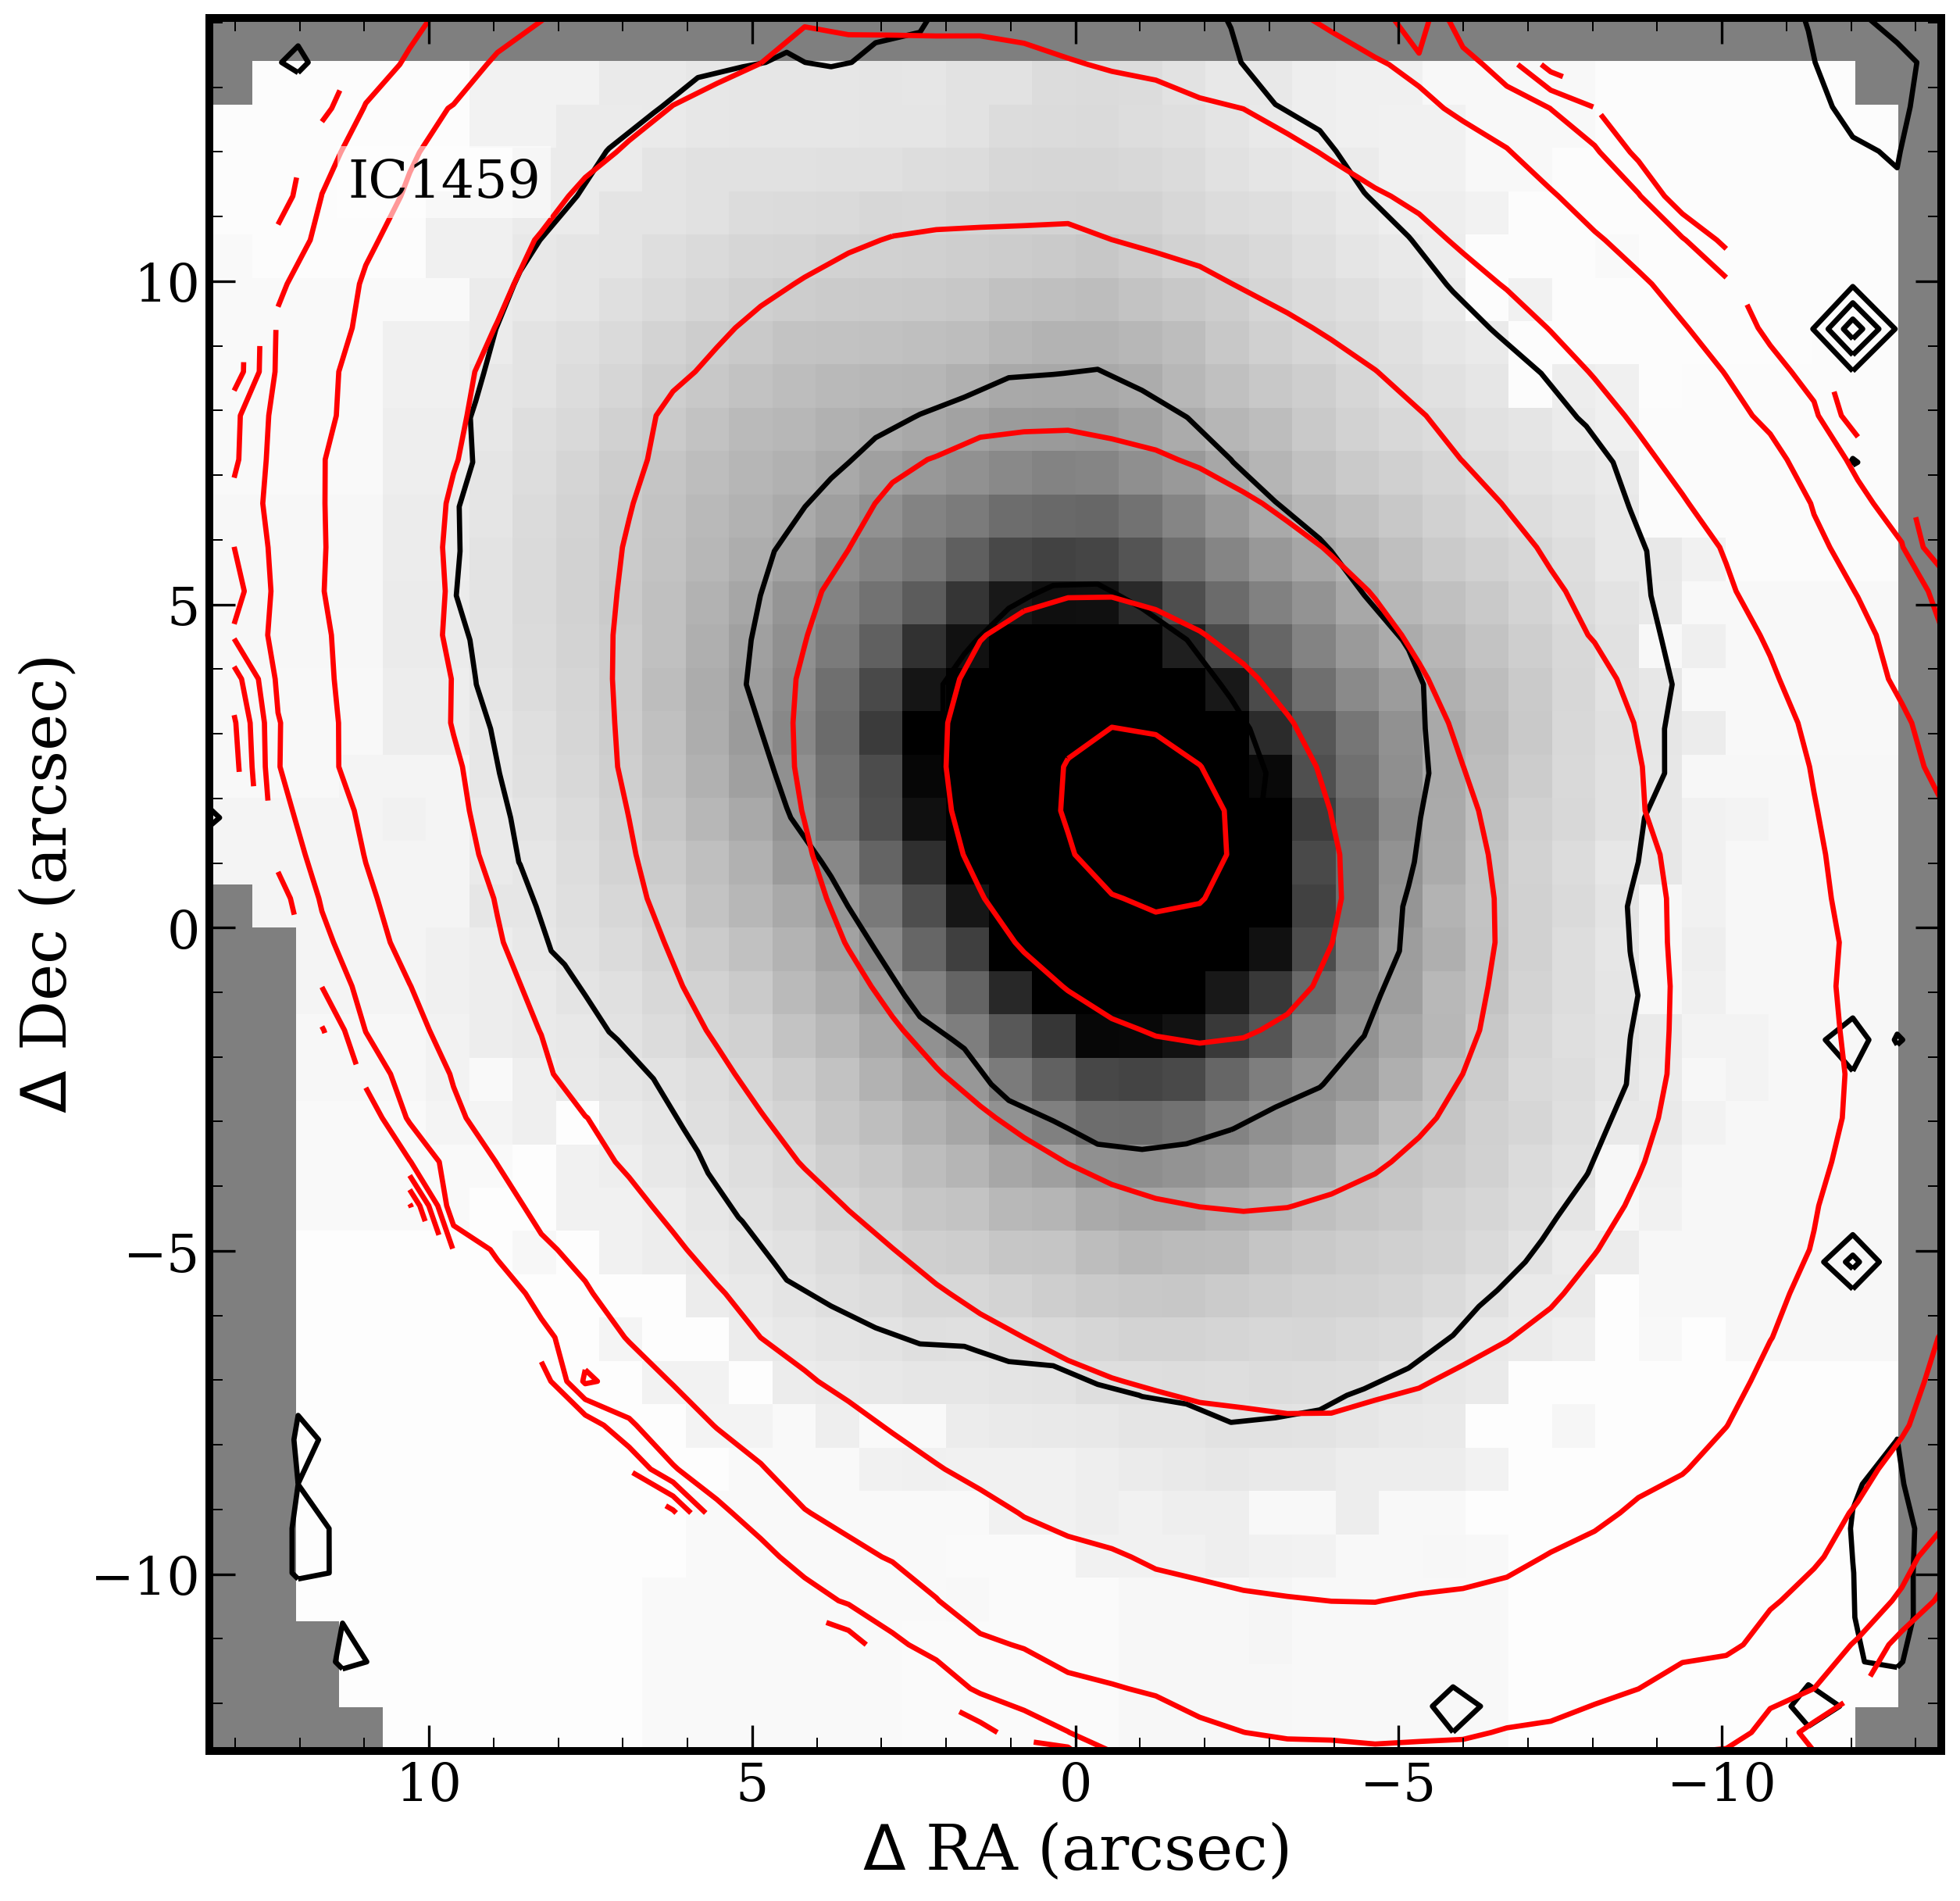
\includegraphics[width=.4\textwidth]{chapter2/hst_vimos_ic1459.png}
			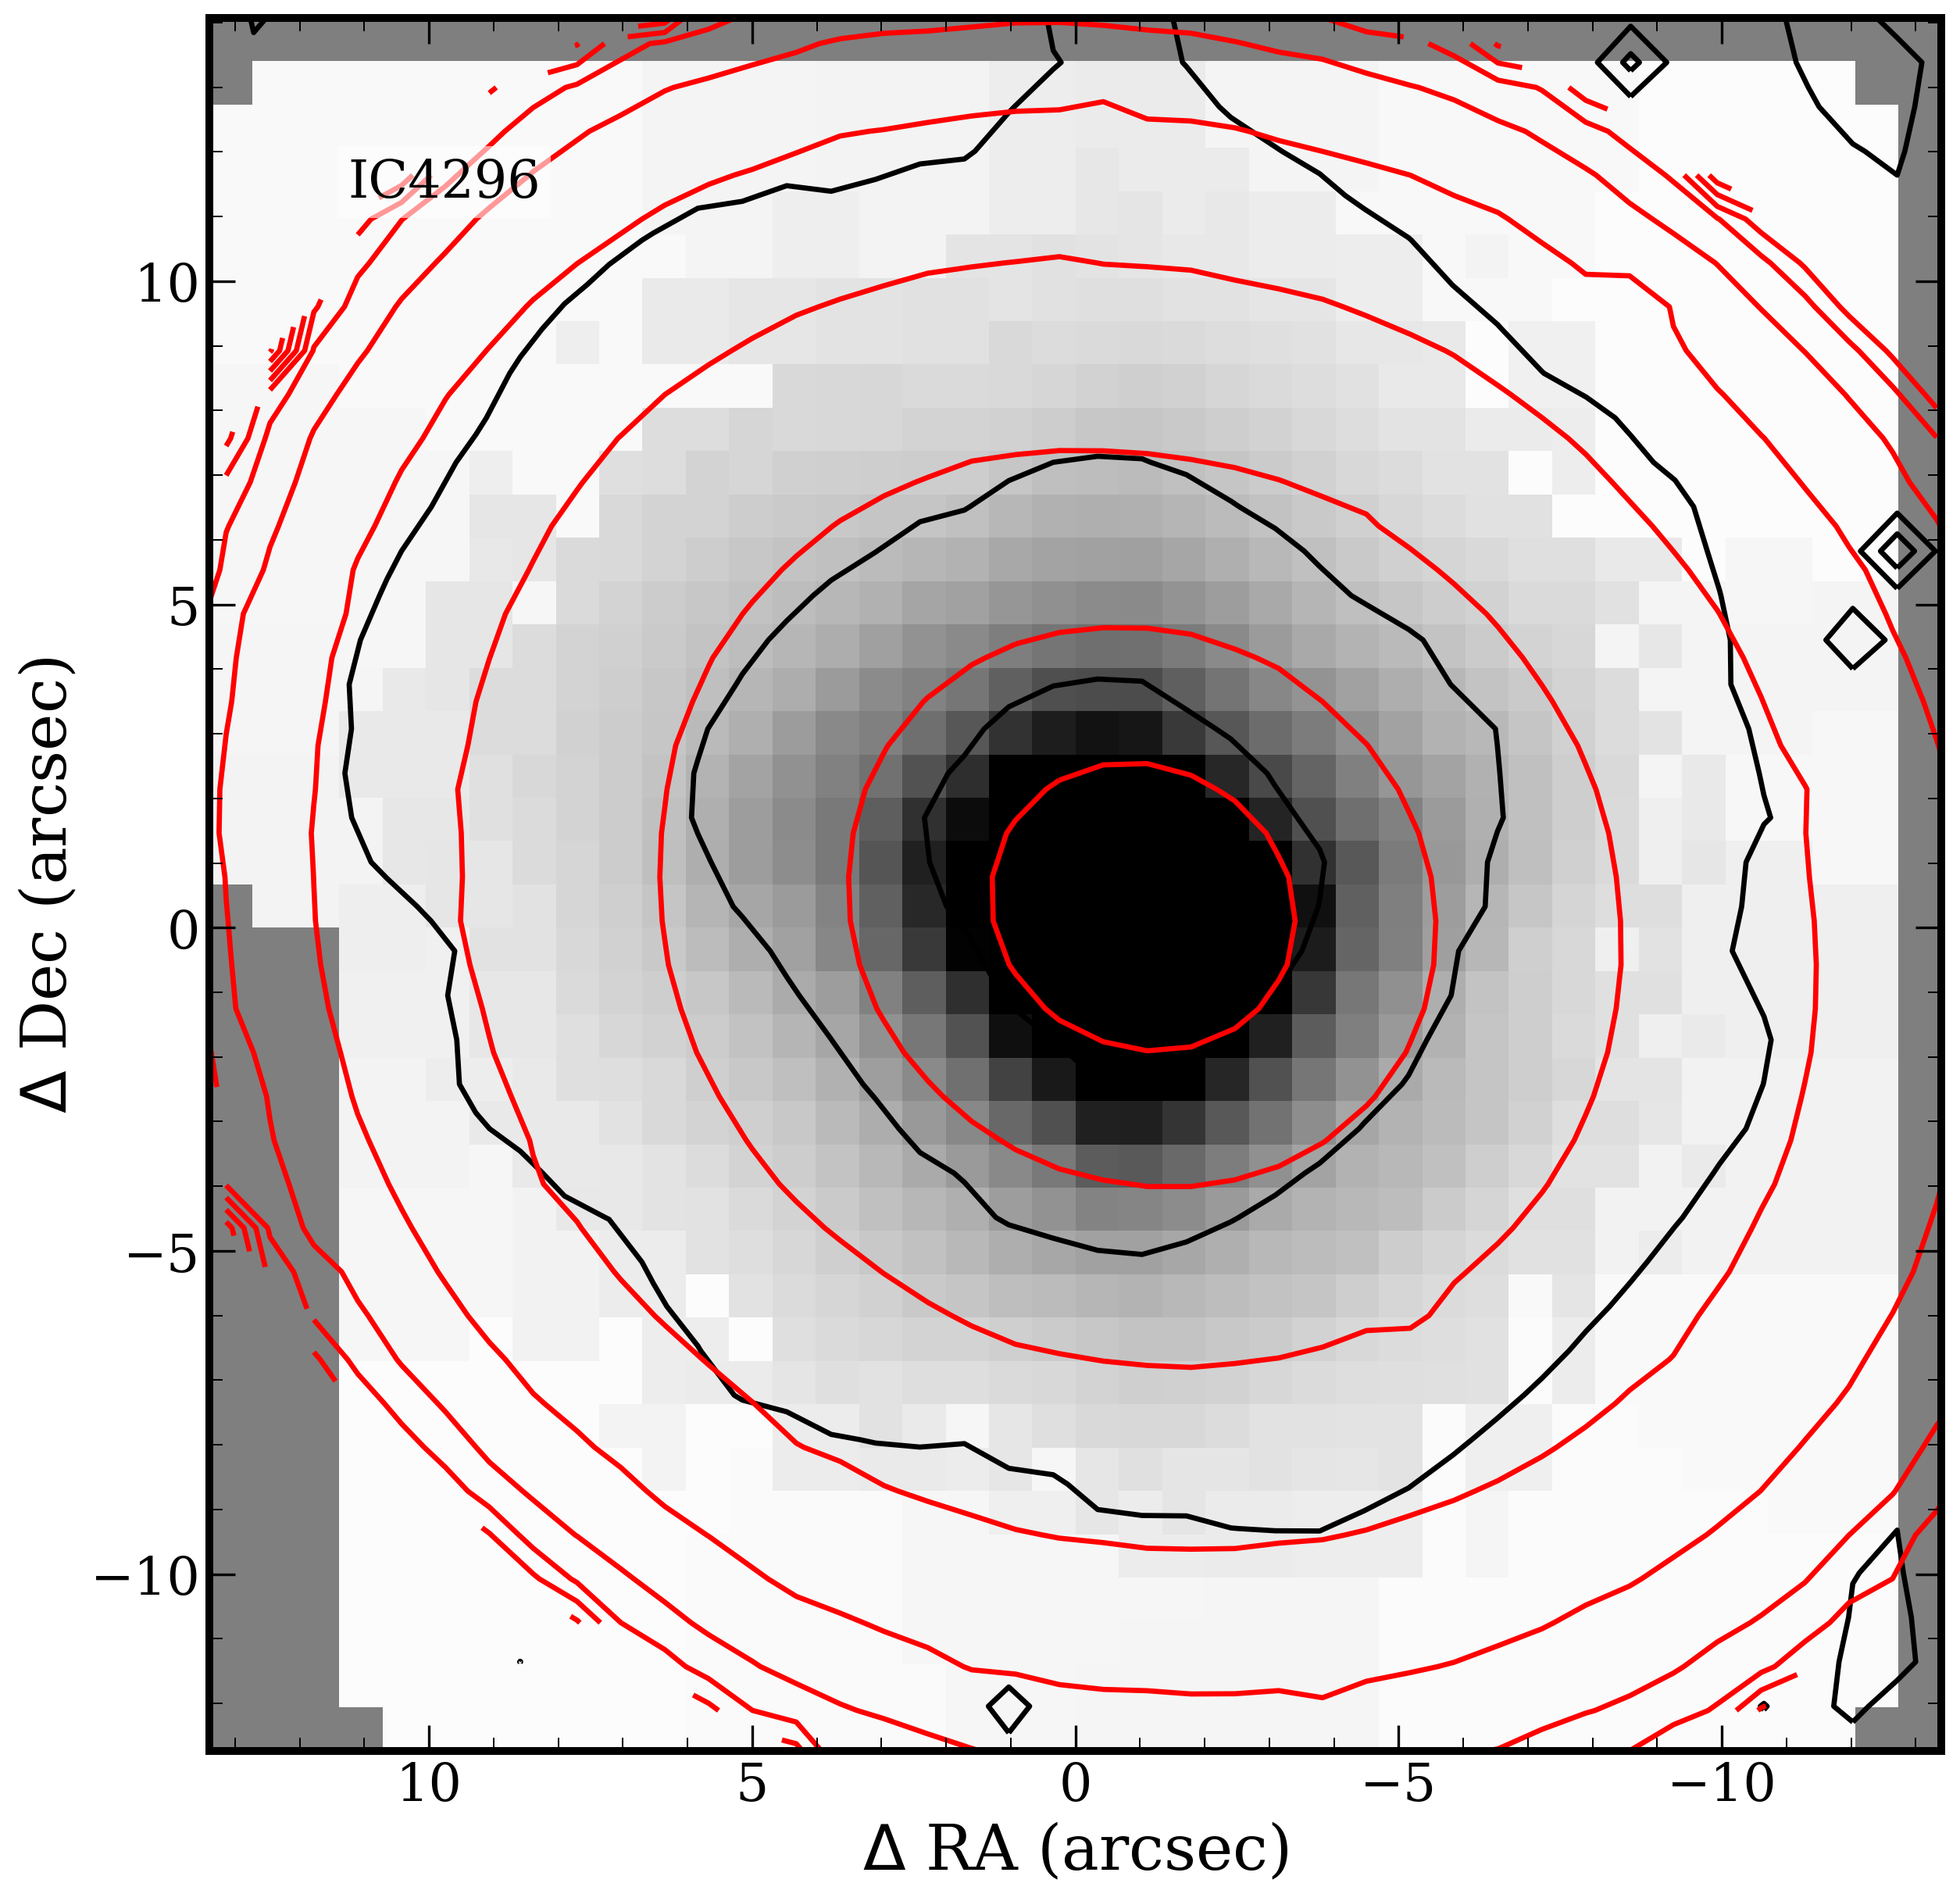
\includegraphics[width=.4\textwidth]{chapter2/hst_vimos_ic4296.png}
			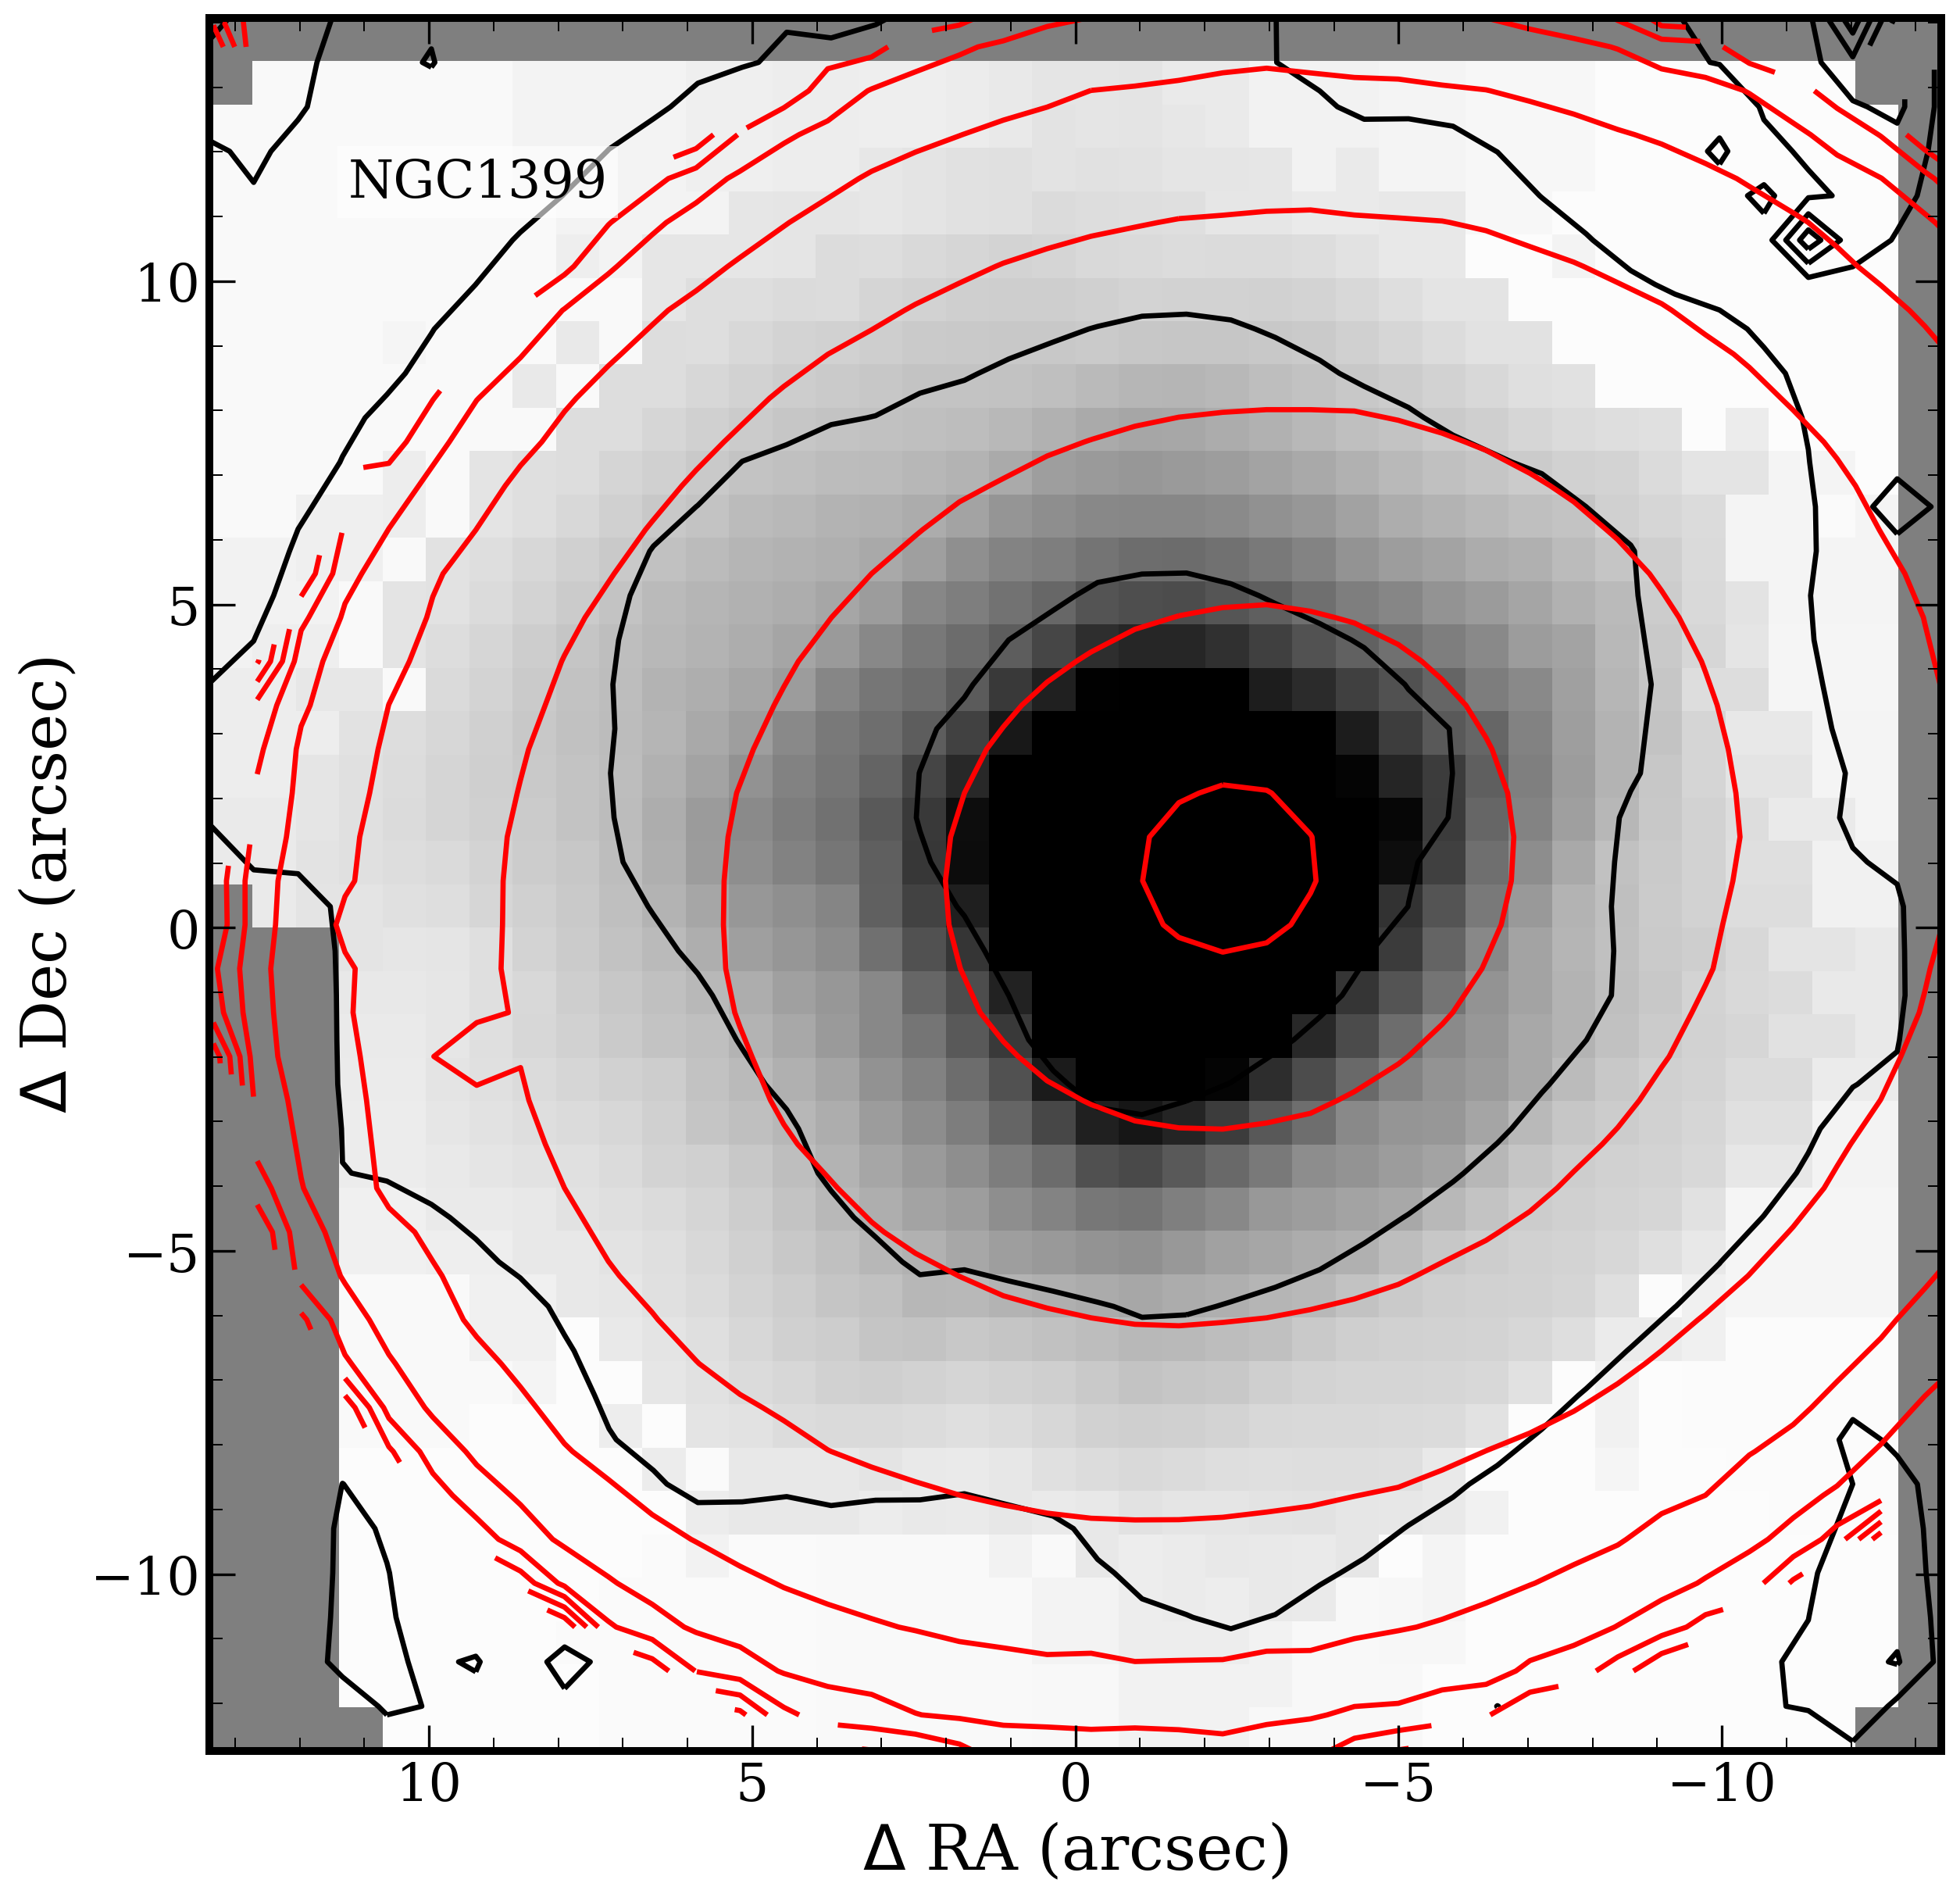
\includegraphics[width=.4\textwidth]{chapter2/hst_vimos_ngc1399.png}
			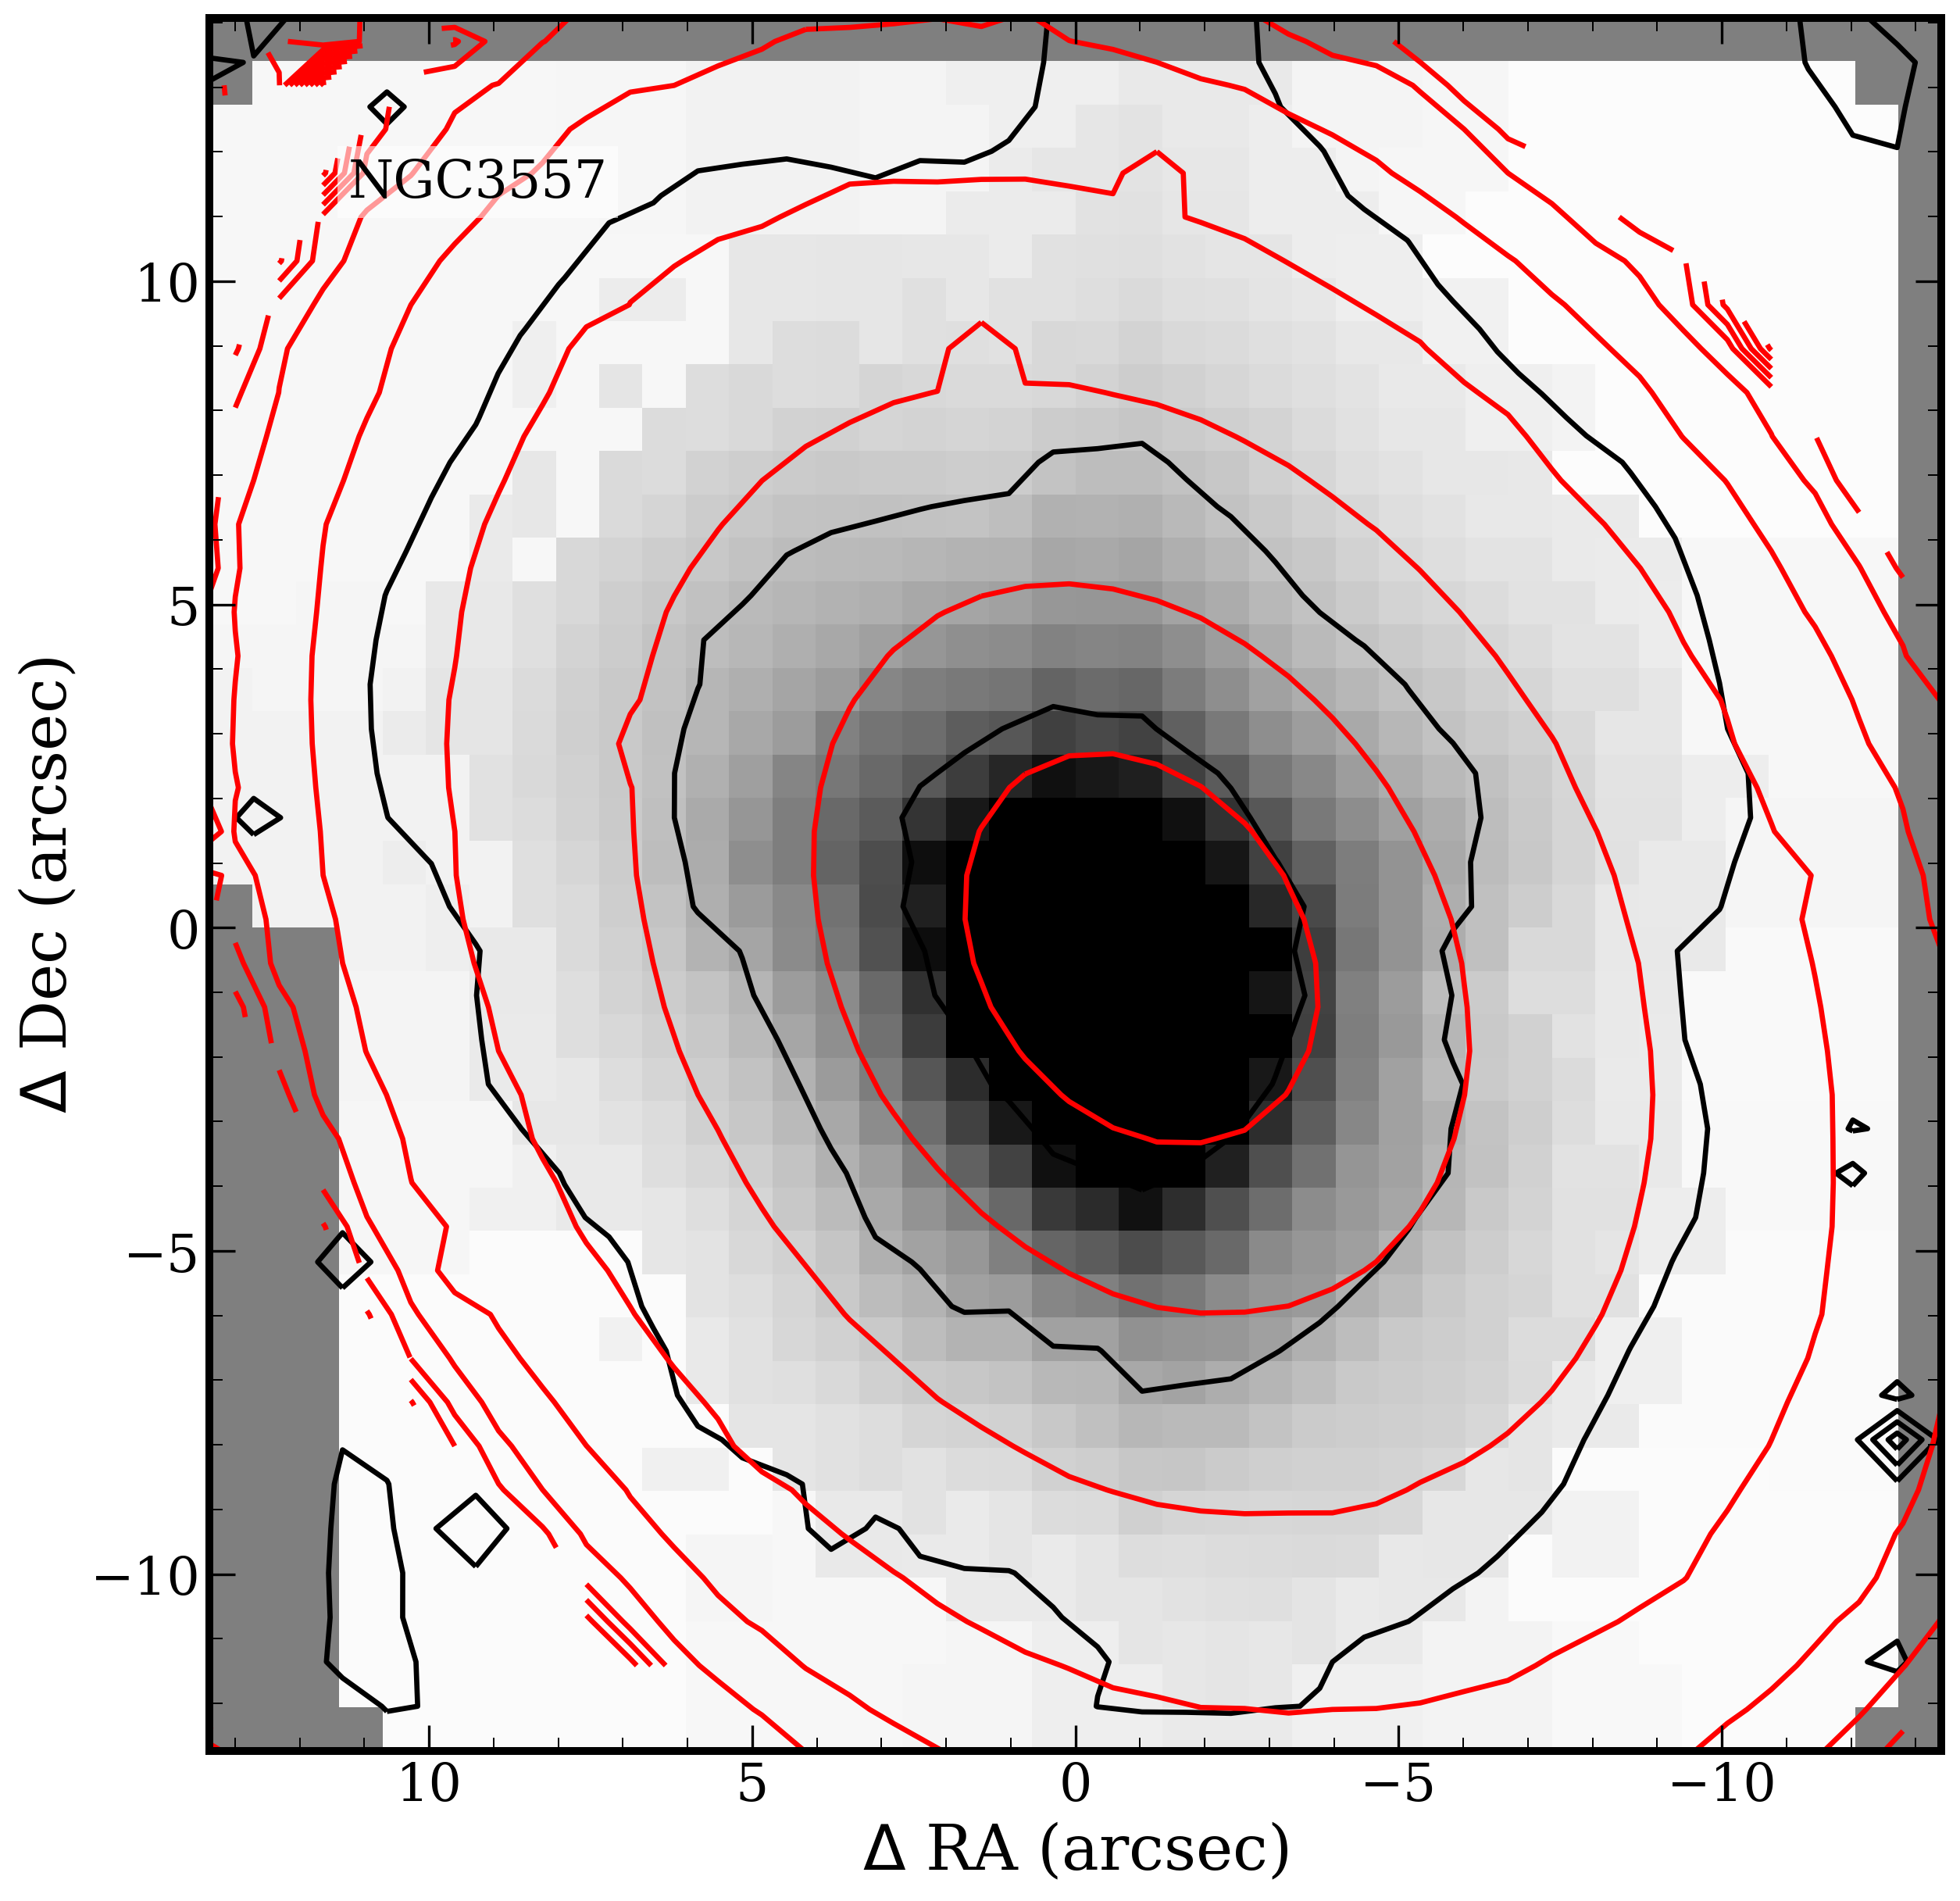
\includegraphics[width=.4\textwidth]{chapter2/hst_vimos_ngc3557.png}
			\caption[Comparison of VIMOS images to \textit{HST}]{Comparison of reconstructed VIMOS image to \textit{HST} image. Clockwise from top left: IC 1459, IC 4296, NGC 3557, NGC 1399. Image and black contours show the VIMOS reconstructed image. Red contours show the \textit{HST} image, reduced to the resolution of VIMOS. All contours are spaced at intervals of 1 mag.}
			\label{fig:HSTvsVIMOS}
		\end{figure}

		The correction spectra found in the process of removing the fringe-like pattern above introduces spatial covariance by effectively applying a spatially smoothing of the data over a scale of 2--3 spaxels. However the effect should not be large, however, so we chose to neglect these correlations and scale the variance spectra by the same factors as the observed spectra. This smoothing is, however, particularly undesirable at the centres of our sample galaxies, where the impact of active galactic nuclei (AGN) should be observed. This should be taken into account later, particularly in Chapter \ref{cha:gas}.

		Finally, in Fig.\,\ref{HSTvsVIMOS} we compare the reconstructed image to \textit{Hubble Space Telescope (HST)} archival images for the four galaxies for which such data existed (IC 1459, IC4296, NGC 1399 and NGC 3557). The \textit{HST} contours (red) are much smoother than the VIMOS contours (black), despite the resolution of the \textit{HST} images being reduced to that of VIMOS. Except for IC 1459 (top left), the VIMOS contours have a characteristic diamond shape due to the poor calibrations between quadrants, which is not seen in the \textit{HST} contours. As stated above, IC 4296 and NGC 1399 are the VIMOS datacubes most effected by the poor quadrant calibrations, while IC 1459 is one of the least effected.

		


	\subsection{Other VIMOS Pipelines}
		\label{subsec:Other}
		Two other publicly available data-reduction pipelines exist for VIMOS. First, the ESO supplied VIMOS pipeline recipe, a plug-in for ESO's general purpose data handling tool \textsc{Gasgano}\footnote{\url{http://www.eso.org/sci/data-processing/software/gasgano}} \citep{Izzo2004, ESO2012}. At the start of this project, this pipeline was not well received by the community. Indeed, ESO's support team suggested I try the alternative pipeline, \textsc{P3D}. Upgrades have since been made to both the instrument and the pipeline, as well as improved suggestions for the observing strategies (OBs), that are meant to remove some of the calibration issues discussed here. However, given the periods when all data were obtained, we have nevertheless decided not to experiment with this tool.
		
		% No publication paper for IDL? Is this because it is commerical?
		Second, \textsc{P3D}\footnote{\url{http://p3d.sourceforge.net/}} is a comprehensive, multi-instrument package with both a decent graphical user interface (GUI) and an application programming interface (API) in the commercial \textsc{Interactive Data Language}\footnote{\url{http://www.harrisgeospatial.com/SoftwareTechnology/IDL.aspx}} (\textsc{IDL}) \citep{Sandin2010, Sandin2011}. It includes routines for all the standard reduction steps: bias subtraction, tracing of the fibres along the dispersion axis, flatfielding, wavelength calibration, flux calibration, cosmic-ray removal and DAR correction. It also combines the quadrants into a single FITS file, although as mentioned above the flux calibration of the different quadrants is attempted by comparing the intensities of the blended sky line at 5199\,\AA. In our case, this calibration step failed for most galaxies as the 5199\,\AA\ sky line is extremely faint (or not detected) in many of the exposures. This failure can be seen in the extremely sharp offsets between the quadrants on the left and right of the reconstructed image shown in the left panel of Fig.\,\ref{fig:P3D}. 

		\begin{figure}
			\centering
			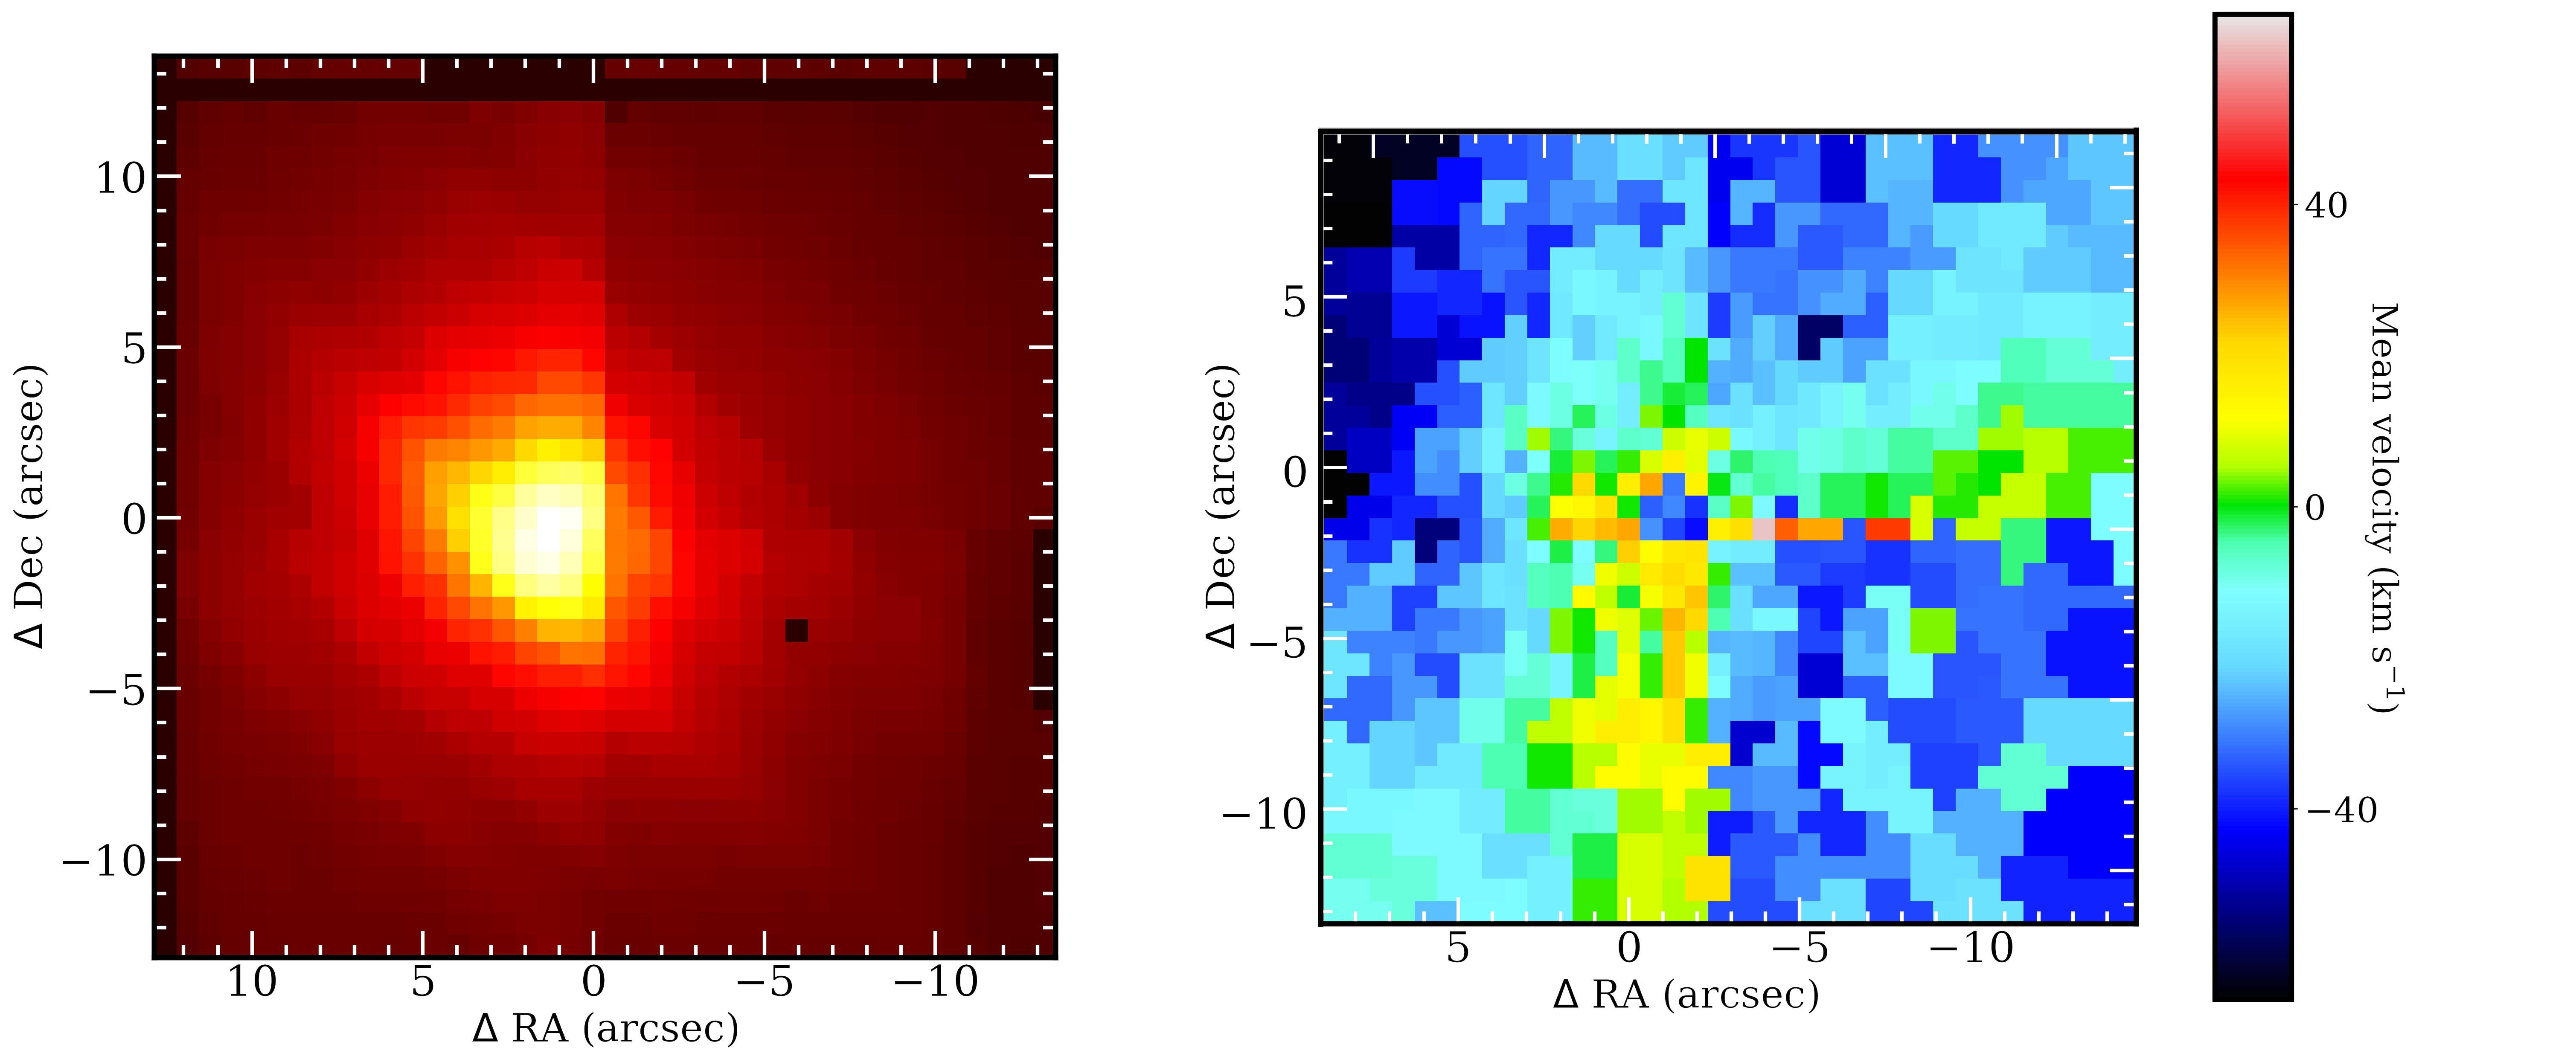
\includegraphics[width=.9\textwidth]{chapter2/P3D_NGC1399.png}
			\caption[\textsc{P3D}-reduced data problems]{Examples of problems with \textsc{P3D}-reduced data. Left panel: flux map (reconstructed image) of NGC 1399 Right panel: mean stellar velocity map of NGC 1399. Both maps show sharp offsets between the quadrants. The outer 2 spaxels on all sides of the velocity map were discarded.}
			\label{fig:P3D}
		\end{figure}


		The \textsc{p3d} wavelength-calibration step was not very successful either, as sharp offsets remain between the quadrants in the spectral direction. While this was still the case with \textsc{Py3D}-reduced data, the issue was much worse and more prevalent for \textsc{P3D}-reduced data. For example, the right panel of Fig.\,\ref{fig:P3D} shows the mean stellar velocity map of NGC 1399 extracted from \textsc{P3D}-reduced data. The wavelength calibration is so poor that the rotation pattern of the galaxy is completely obfuscated.

		
\section{Multi-unit Spectroscopic Explorer (MUSE)}
	\label{sec:MUSE}

	\subsection{MUSE Instrument}
		The Multi-unit Spectroscopic Explorer (MUSE) is located on UT4 of ESO's VLT \citep{Bacon2010}. It is comprised of 24 channels, each feeding an IFU (image slices) and spectrographs for a total contiguous field of view of $1\arcmin \times 1\arcmin$ at spatial sampling of $0\farcs2$. It has a spectral range of 4800-9300\,\AA\ with a spectral resolution of $\approx 2.3$\,\AA\ sampled at 1.25\,\AA\,pix$^{-1}$. MUSE is currently offered with and without adaptive optics (AO), and a narrow-field mode (with an order of magnitude improvement in spatial resolution and sampling) is planned for the future. 
		
	\subsection{MUSE Archival Observations}
		Four of the sample galaxies are in the MUSE archive: IC 1459, IC 4296, NGC 1316 and NGC 1399. NGC 1316 (observed as part of programme 094.B-0298A) and NGC 1399 (programme 094.B-0903A) were both observed as mosaics, while IC 1459 and IC 4296 (both also programme 094.B-0298A) were observed in single pointings. All were observed in service mode during ESO period 94, in the MUSE wide-field mode without adaptive optics. Every OB in both programmes followed the standard MUSE calibration plan.

	\subsection{MUSE Data Reducing}
		\label{subsec:MUSEreduction}
		
		Because the computing resources required to reduce raw MUSE data are very large (the recommended system configuration for the reduction of a single-pointing OB of 5 exposures is: 64\,GB of memory, 24 CPU cores and 4\,TB of free disk space), the data quality is high, and the pipelines products are known to be robust, we adopt for this project the pre-reduced (known as Phase 3) data products from ESO, so that the ESO data reduction pipeline\footnote{\url{http://www.eso.org/sci/software/pipelines/muse/muse-pipe-recipes.html}} is already applied. 

		The ESO pipeline contains all standard IFU data reduction steps: bias subtraction, flatfielding of detectors using continuum lamp exposures, flatfielding of fibres using twilight exposures, wavelength calibration, flux calibration using standard stars and sky subtraction (both programmes included dedicated sky exposures). Tiled observations, where present, are combined into a final mosaic.

		We found that the Phase 3 data products were indeed generally of a sufficient quality for our purposes, except that in both IC 1459 and IC 4296 the sky appears to have been over-subtracted. The ESO Phase 3 data release description for MUSE\footnote{\url{https://www.eso.org/sci/observing/phase3/data\_releases/IDP\_MUSE\_IFU\_release\_description\_1.0.pdf}} points out that the automatic data-reduction routine does not verify stable conditions (such as photometry and moon visibility) before applying the sky subtraction. Unstable conditions may well be the source of over subtraction which manifested itself as enormous apparent absorption features (often with negative fluxes) in the spectra. To remove this over-subtraction, we developed our own pseudo-sky subtraction routine. A median spectrum was taken from four $20 \times 20$\,spaxel regions, one in each spatial corner of the ESO reduced cube. After checking that no stellar continuum could be fit to the medium sky spectrum (i.e.\ that very little light from the galaxy is contaminating the pseudo-sky regions), this median sky spectrum was subtracted from each spaxel in the cube. 

		This extra (pseudo-)sky subtraction was not possible for NGC 1316 and NGC 1399 due to mosaic nature of the observations, since this sky subtraction should be applied to each exposure of the mosaics independently (while the different exposures are already combined as part of the automated data reduction). It is also impossible to access data products from intermediate steps in the data-reduction process, such as immediately before the mosaic is produced. Fortunately, both NGC 1316 and NGC 1399 are not as badly affected by poor sky subtraction as IC 1459 and IC 4296, so they are left uncorrected. 

		Finally, we trimmed all the cubes to the central $30\arcsec \times 30\arcsec$ ($150 \times 150$\,spaxels) only, to (a) avoid the regions used for the pseudo-sky spectrum and (b) reduce the computing resources required for spatial binning (see Section \ref{sec:analysis}). In any case, the bins would be so large in the outer parts as to be effectively useless (see Fig\,\ref{fig:egSNR}).

		As for the VIMOS data, the variance spectra are propagated throughout the entire data-reduction pipeline, including our additional pseudo-sky subtraction step, and are squared-rooted at the end, to be used as noise inputs at the analysis stage. 

		\subsubsection{MUSE Data Quality}
			As with the VIMOS data, we here (Fig.\,\ref{fig:HSTvsMUSE}) examine the reconstructed images (image and black contours), with archival \textit{HST} images (red contours). All galaxies in our sample for which MUSE data was available, also had archival \textit{HST} images available too. It can clearly be seen that the MUSE contours well match the \textit{HST} contours, unlike the for the VIMOS data (see Fig.\,\ref{fig:HSTvsVIMOS}). As such, it can be seen that the MUSE data is of a superior quality to the VIMOS data and as such, where both are available, a higher weighting should be given the MUSE data and its derivatives. 

			\begin{figure}
				\centering
				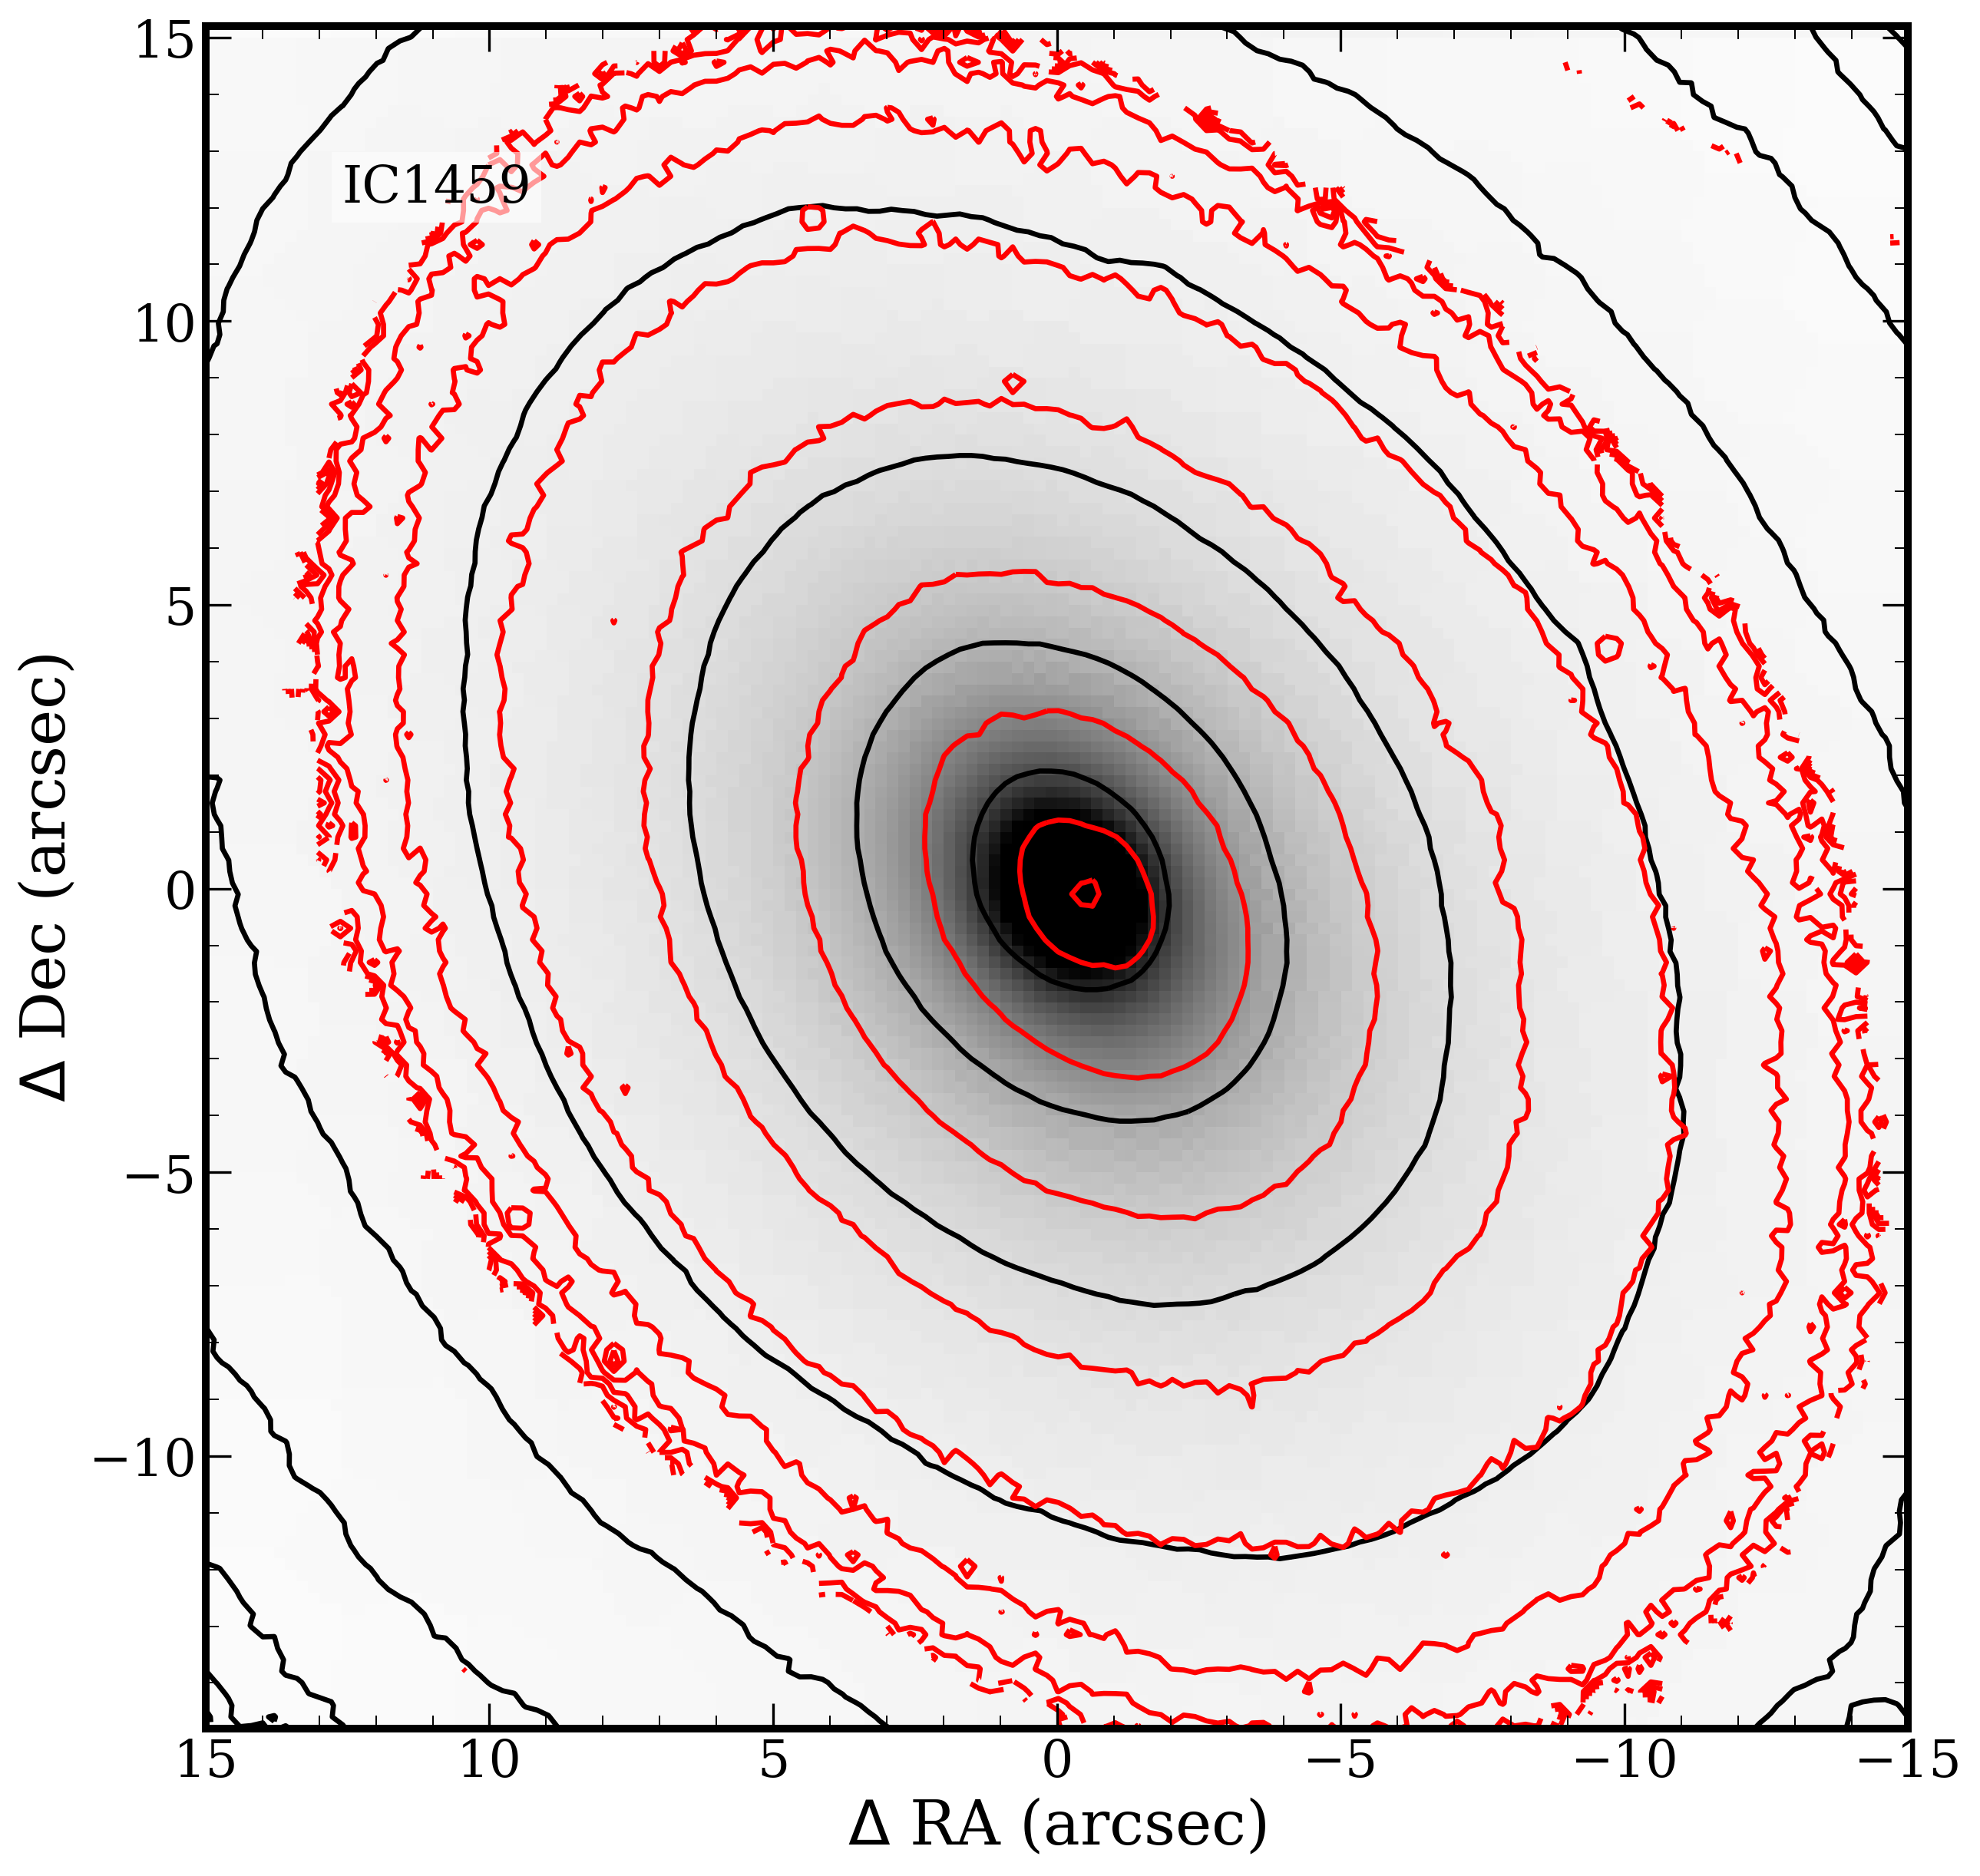
\includegraphics[width=.4\textwidth]{chapter2/hst_muse_ic1459.png}
				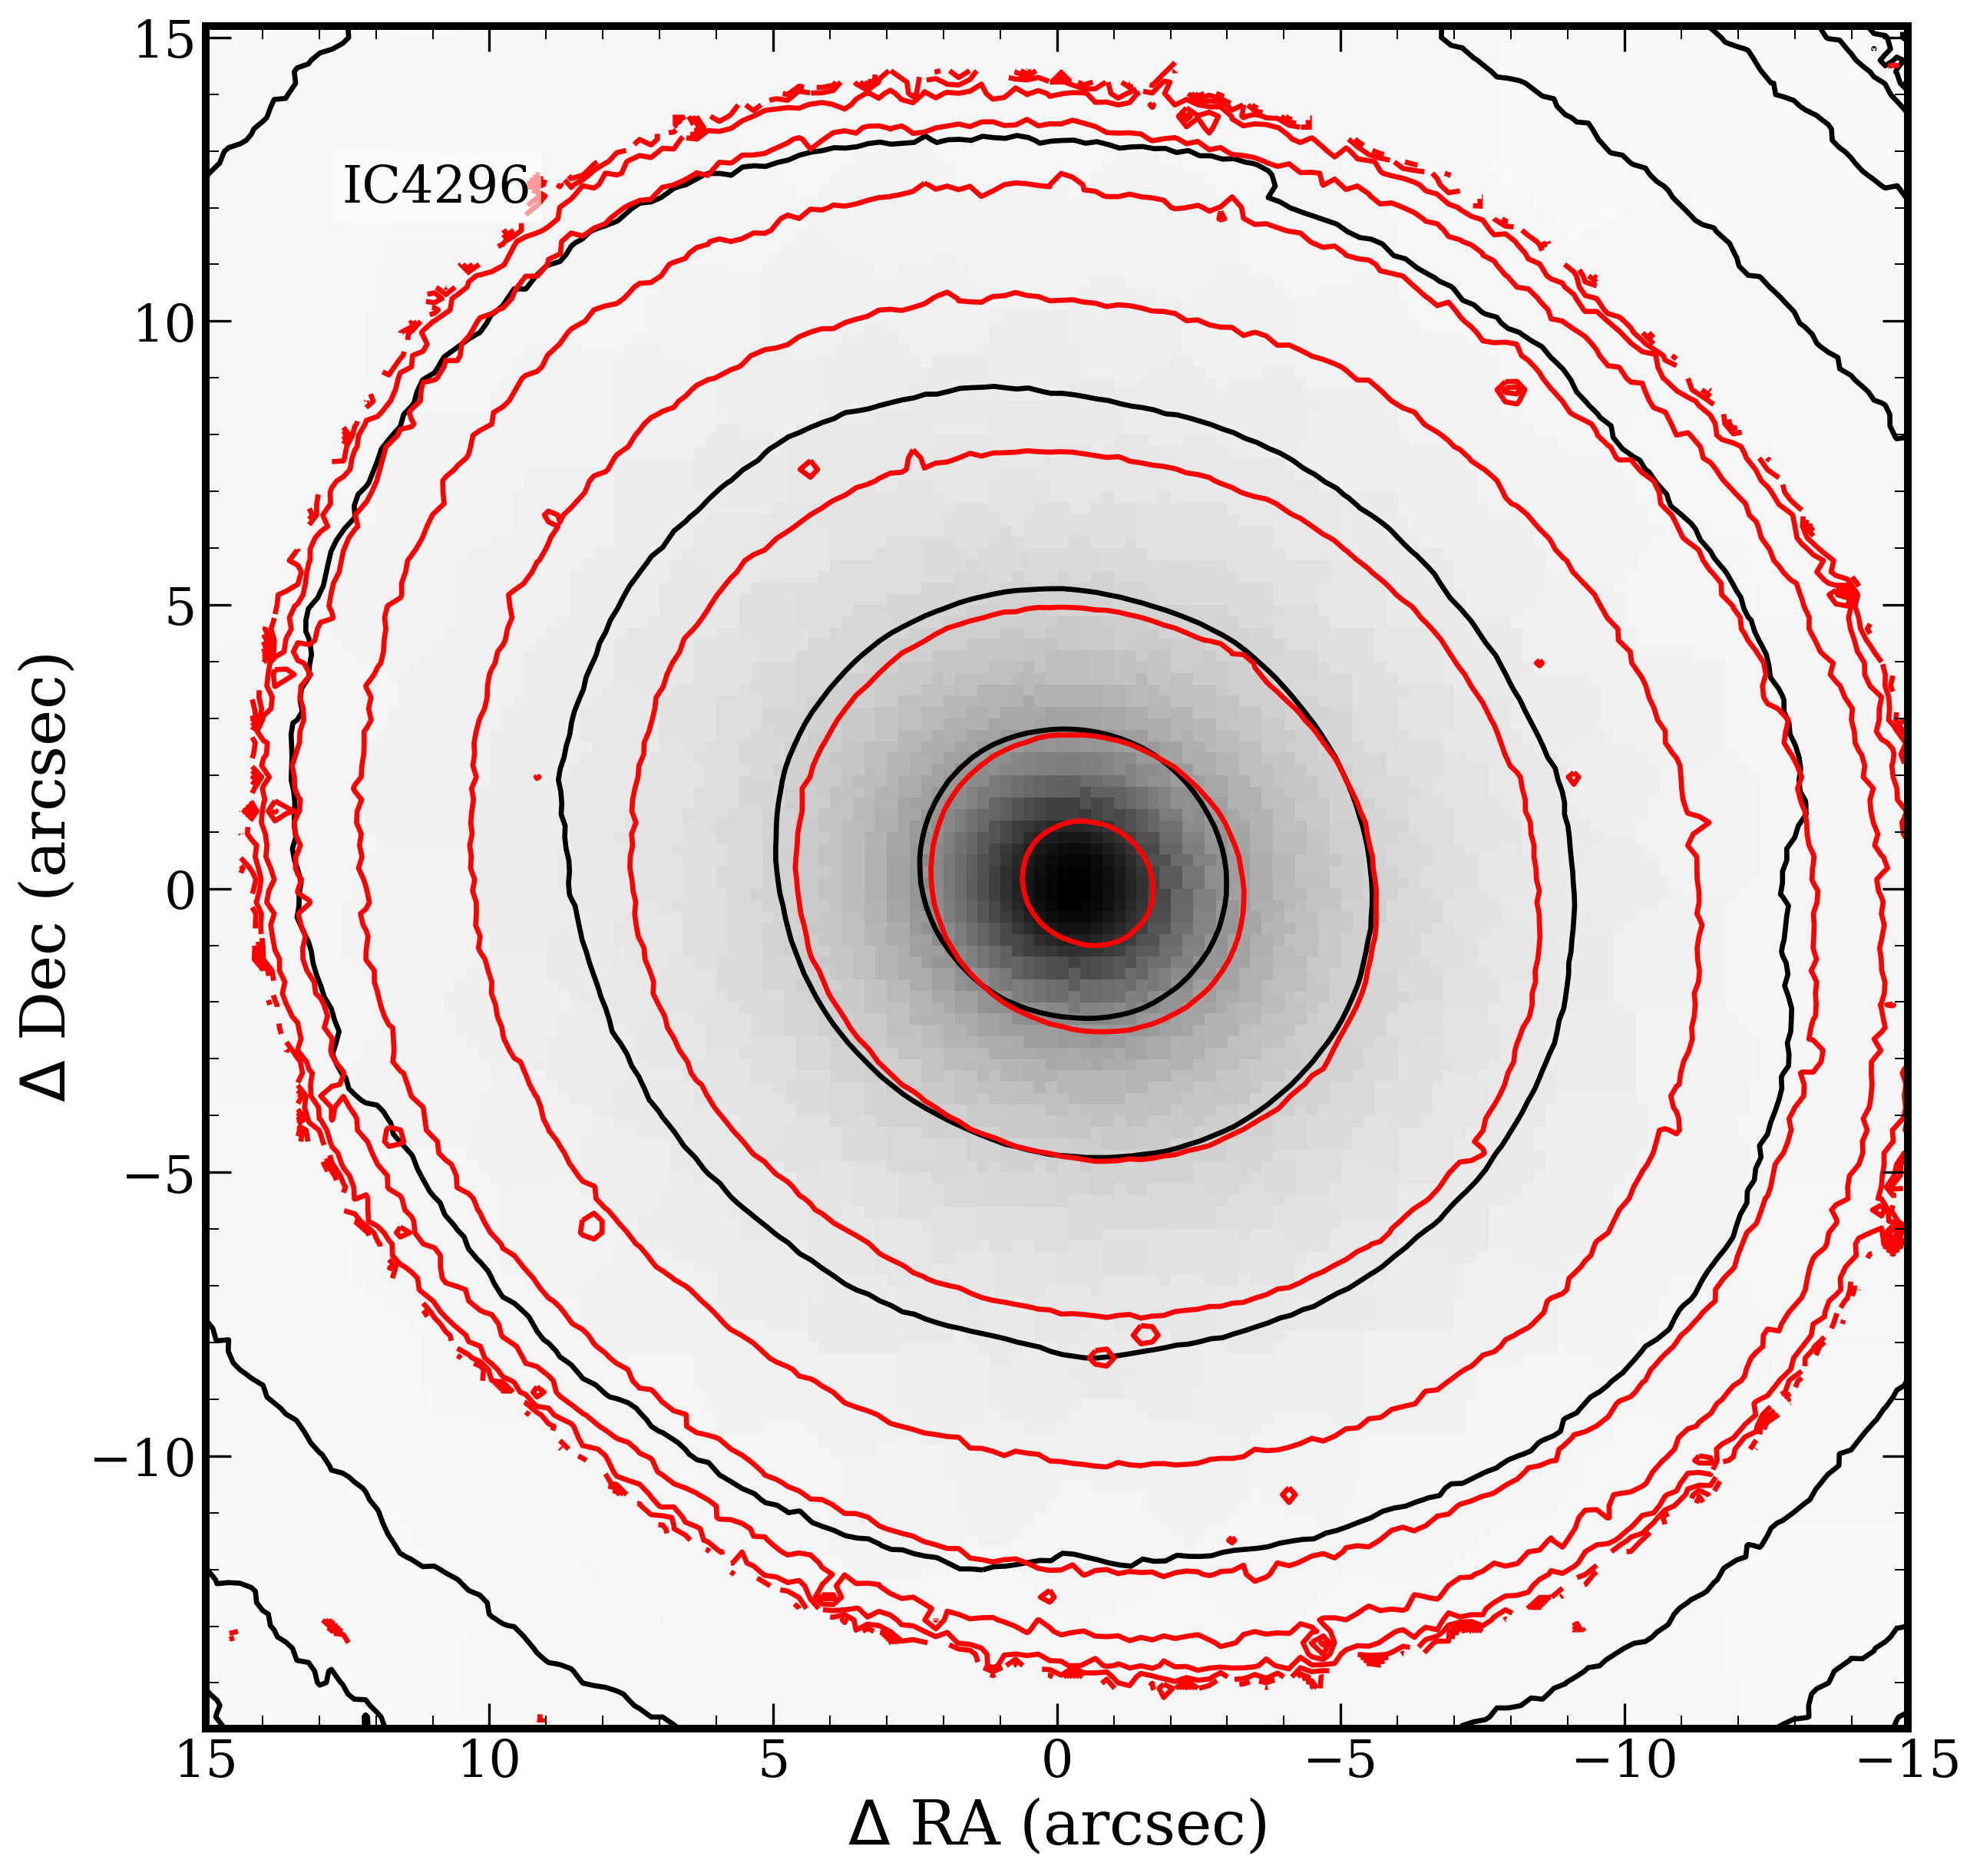
\includegraphics[width=.4\textwidth]{chapter2/hst_muse_ic4296.png}
				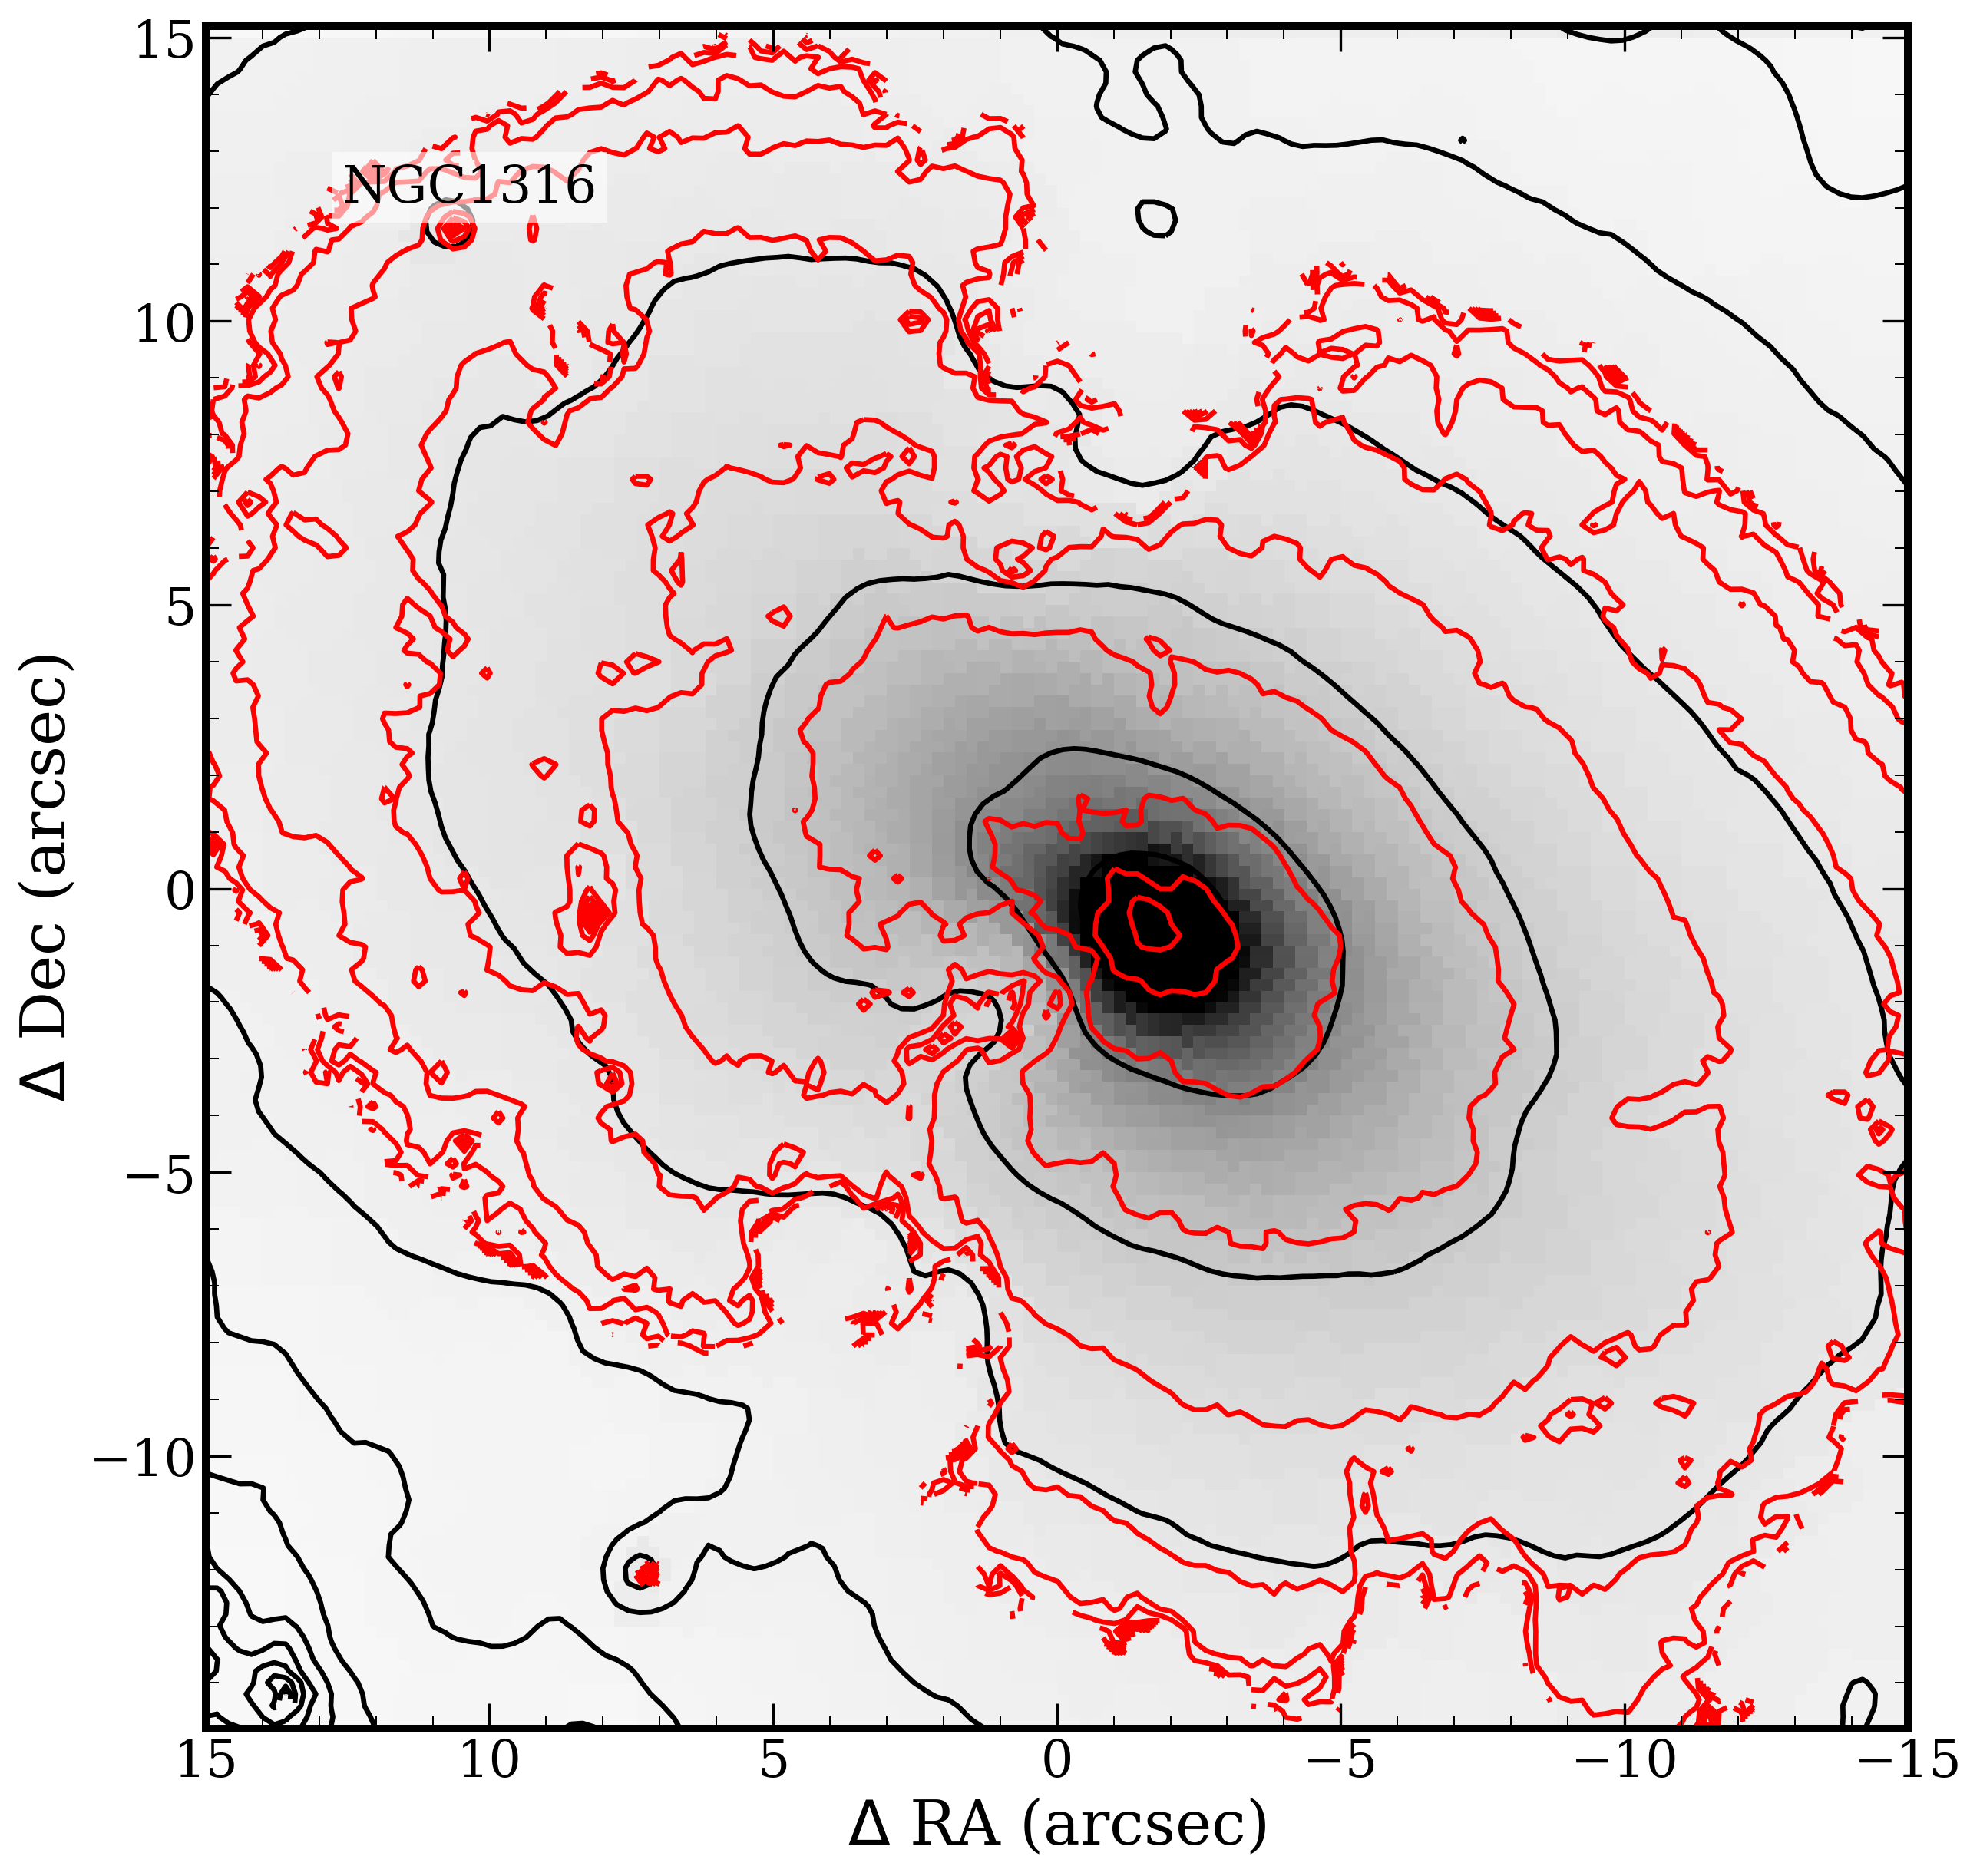
\includegraphics[width=.4\textwidth]{chapter2/hst_muse_ngc1316.png}
				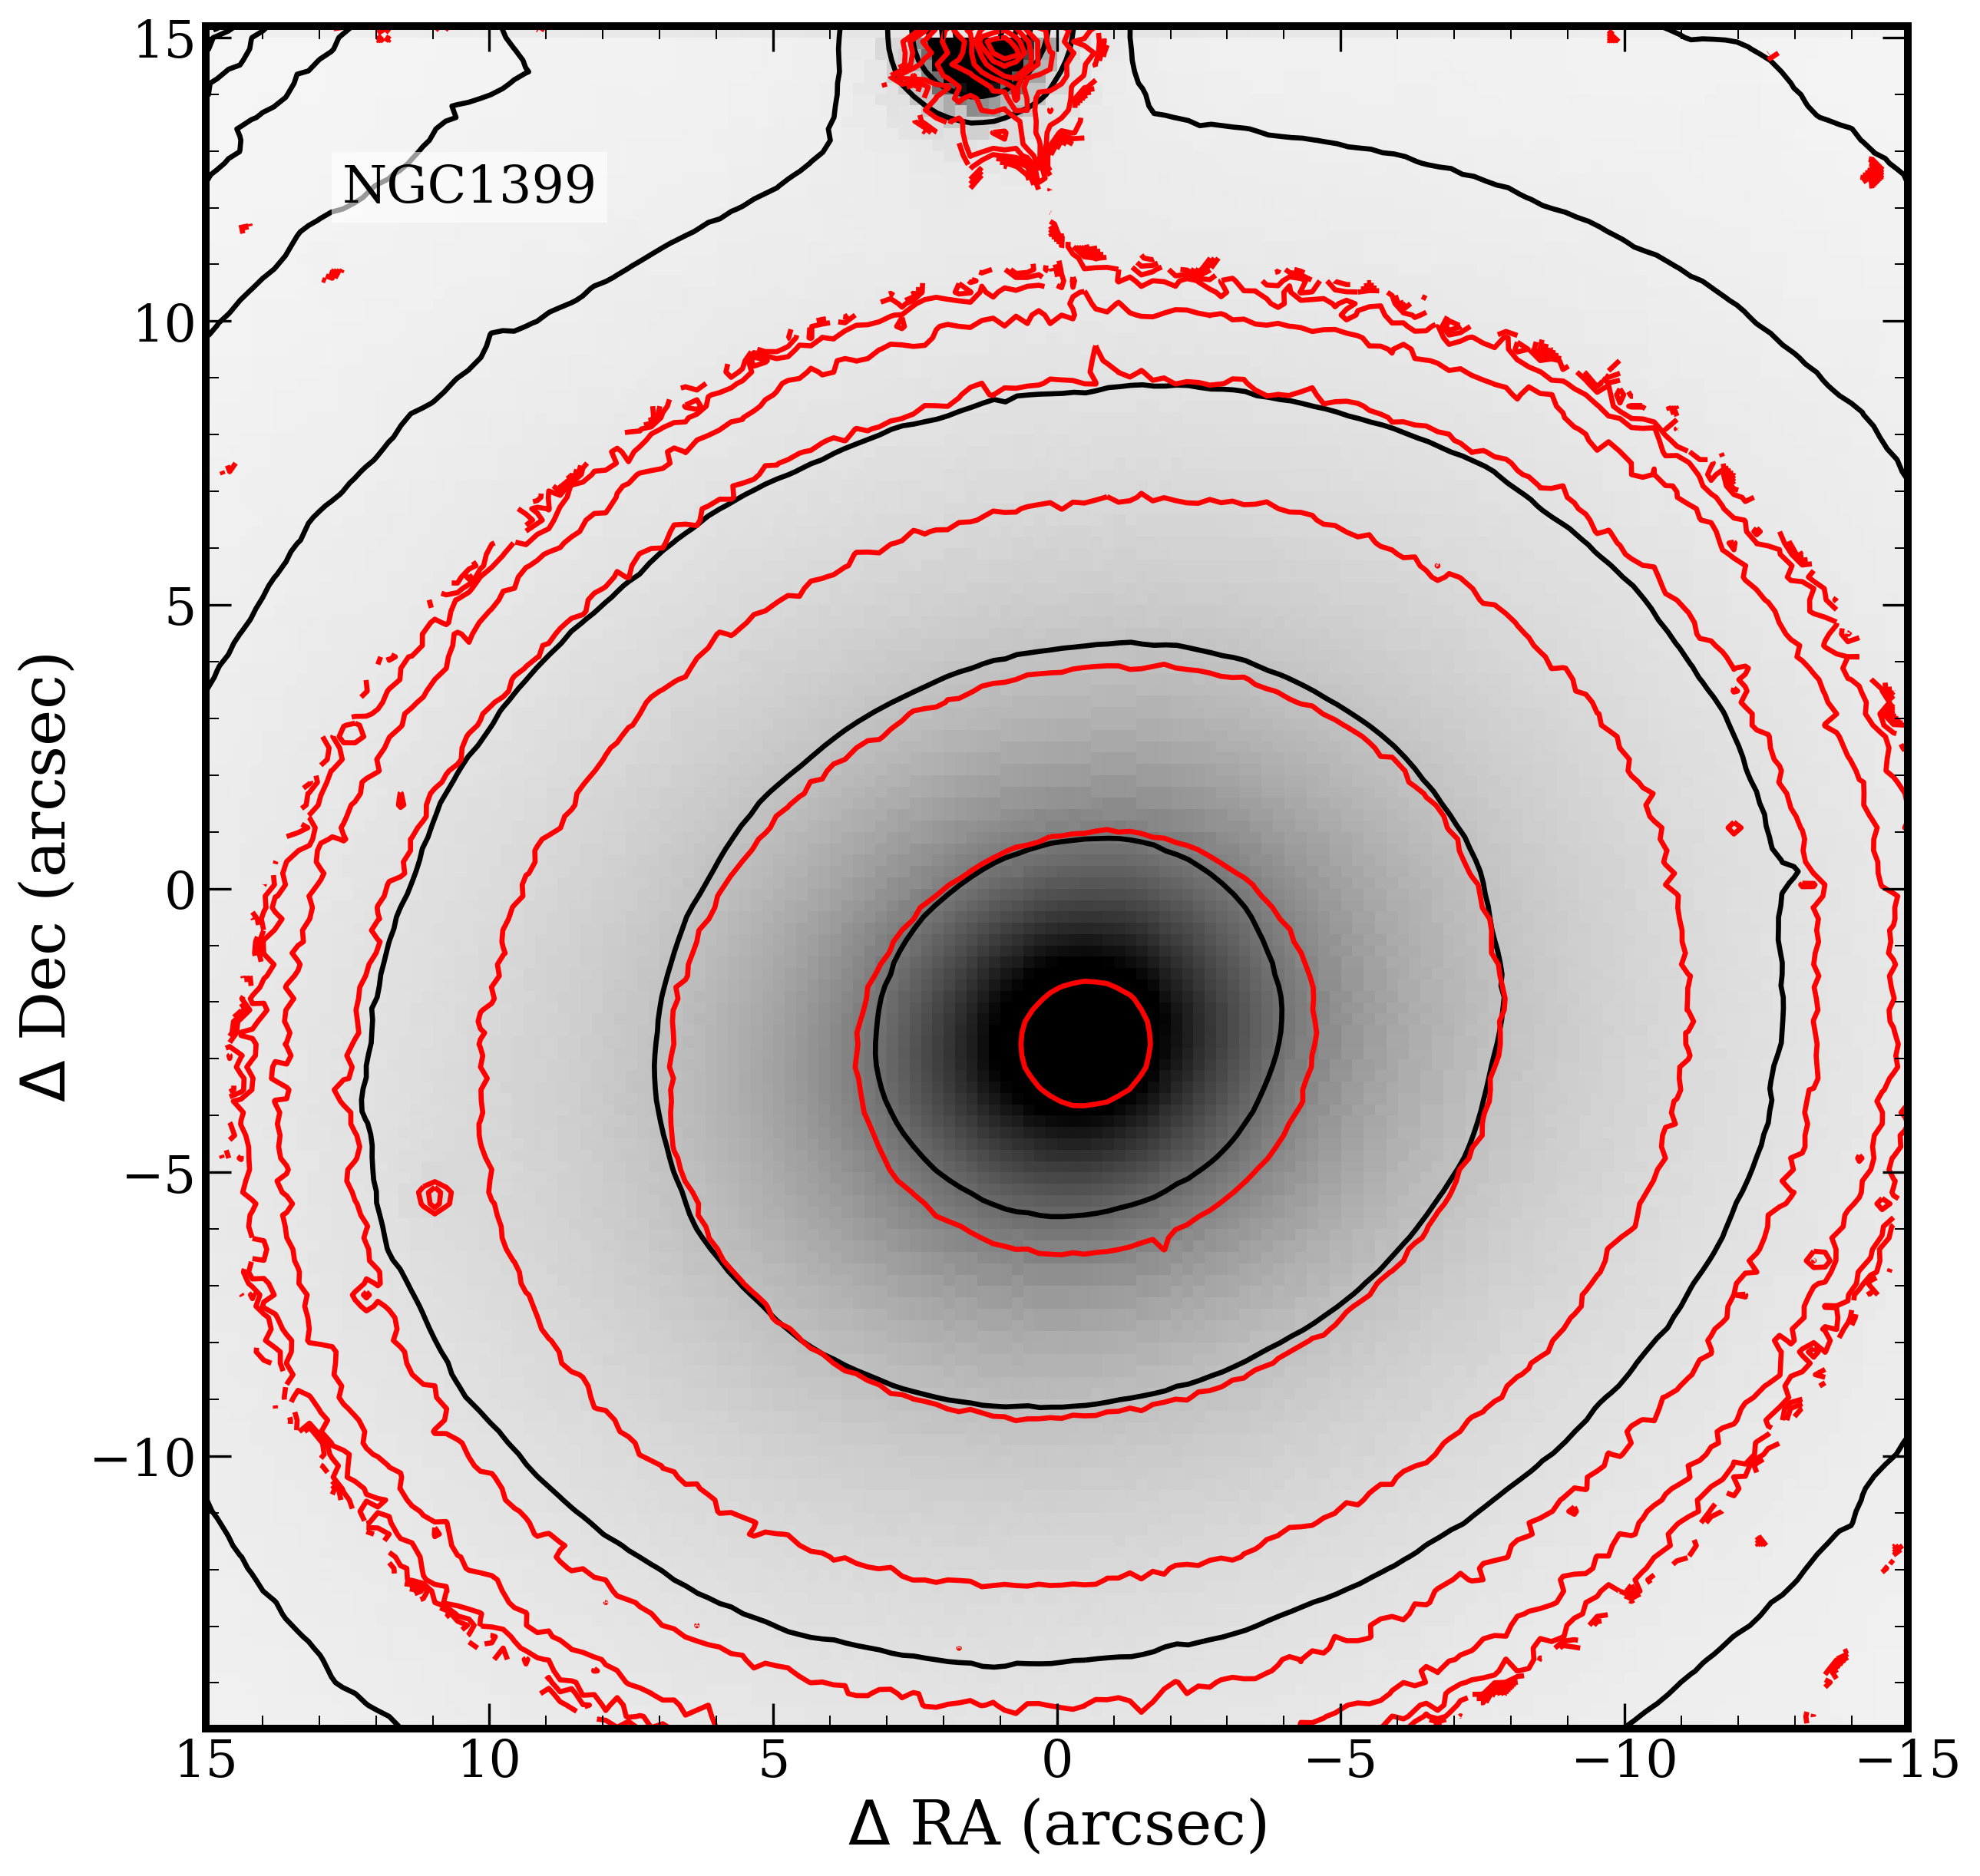
\includegraphics[width=.4\textwidth]{chapter2/hst_muse_ngc1399.png}
				\caption[Comparison of MUSE images to HST]{Comparison of reconstructed VIMOS image to \textit{HST} image. Clockwise from top left: IC 1459, IC 4296, NGC 1316, NGC 1399. Image and black contours show the MUSE reconstructed image. Red contours show the \textit{HST} image, reduced to the resolution of VIMOS. All contours are spaced at intervals of 1 mag.}
				\label{fig:HSTvsMUSE}
			\end{figure}


\section{Data Analysis}
	\label{sec:analysis}
	From this point on, the VIMOS and MUSE datasets are treated almost identically, the only difference (other than the different spectral ranges and resolutions) being that the MUSE datacubes are binned to a higher signal-to-noise ratio (S/N).

	For each galaxy (i.e.\ each combined cube), the data analysis process can be summed up as follows, each step being detailed below:
	\begin{enumerate}
		\item Spatially bin the spectra using Voronoi binning.
		\item Identify the relevant stellar templates, by fitting the entire galaxy spectrum (obtained by summing all galaxy spectra) with all the templates from the Medium-resolution Isaac Newton Telescope (INT) Library of Empirical Spectra (MILES) library, and hereafter using only the non-zero weight templates.
		\item Estimate the redshift and velocity dispersion of the entire galaxy spectrum with an iterative routine. % Markov chain Monte--Carlo (MCMC) routine. 
		\item Find the best-fitting line-of-sight velocity distribution (LOSVD; as parametrised by the Gaussian parameters $v$, the mean velocity and $\sigma$, the velocity dispersion) of the stellar and ionized gas components in each bin, using a Monte--Carlo method to estimate the uncertainties on the measurements. 
		\item Remove the fitted emission lines and measure the absorption line strengths in each bin. 
		\item Identify the best-fitting stellar population model in each bin using the measured absorption line strengths.
	\end{enumerate}

	The results from these pipelines are used in the following chapters to compare the properties and characteristics of our Southern Sample of radio galaxies to those of radio-quiet ETGs. 
	
	\subsection{Spatial Binning}
		\label{subsec:Binning}
		Given that galaxies are brightest at their centres and fade away radially, and that the noise (assumed to be Poisson dominated) scales as the square root of the signal, the S/N of the galaxy spectra will also be highest at the galaxy centres, decreasing with increasing radius. In the outer regions of galaxies, the S/N becomes too low to extract meaningful information from the spectra. Because of this, we spatially bin the spectra to a fixed target S/N (increasing a bin's size until it reaches the required S/N). This is performed using the adaptive Voronoi binning routine\footnote{\url{http://www-astro.physics.ox.ac.uk/~mxc/software/}} of \citet{Cappellari2003}. For our purposes, we define the `signal' and `noise' of each spaxel as the median value of its spectrum and noise spectrum, respectively. We require a S/N of 30 for all VIMOS datacubes and 50 for the IC 1459 and IC 4296 MUSE datacubes. The NGC 1316 and NGC 1399 MUSE datacubes were binned to a S/N of 50 for the analysis of the stellar kinematics and 100 for the analysis of the emission line kinematics and stellar populations. These target S/N were chosen in order to be as low as possible, while still returning meaningful information (as assessed by eye). The NGC 1316 and NGC 1399 MUSE datacubes have different S/N thresholds due to the extra (pseudo-)sky subtraction applied to the IC 1459 and IC 4296 datacubes, that were successful at removing artefacts from the spectra (thus allowing us to retain a higher level of spatial information for these two galaxies). The remaining artefacts in NGC 1316 and NGC 1399 datacubes did not seem to affect the analysis of the stellar kinematics, but did affect the emission line fits, so we enforced a higher S/N threshold for the emission line analysis and where careful subtraction of the emission lines is important (i.e.\ in the analysis of the stellar populations). 

		Figure \ref{fig:egSNR} shows an example of the Voronoi bins. Concentric rings can clearly be seen around the centre of the galaxy, as bins with a S/N just below the target are increased in size by a single spaxel, resulting in a final S/N well over the target. Spaxels within the first ring are not binned and can have arbitrarily high S/N (dictated by the galaxy surface-brightness profile), while bins outside the central rings are composed of many spaxels and naturally have S/Ns clustered around the target value.

		\begin{figure}
			\centering
			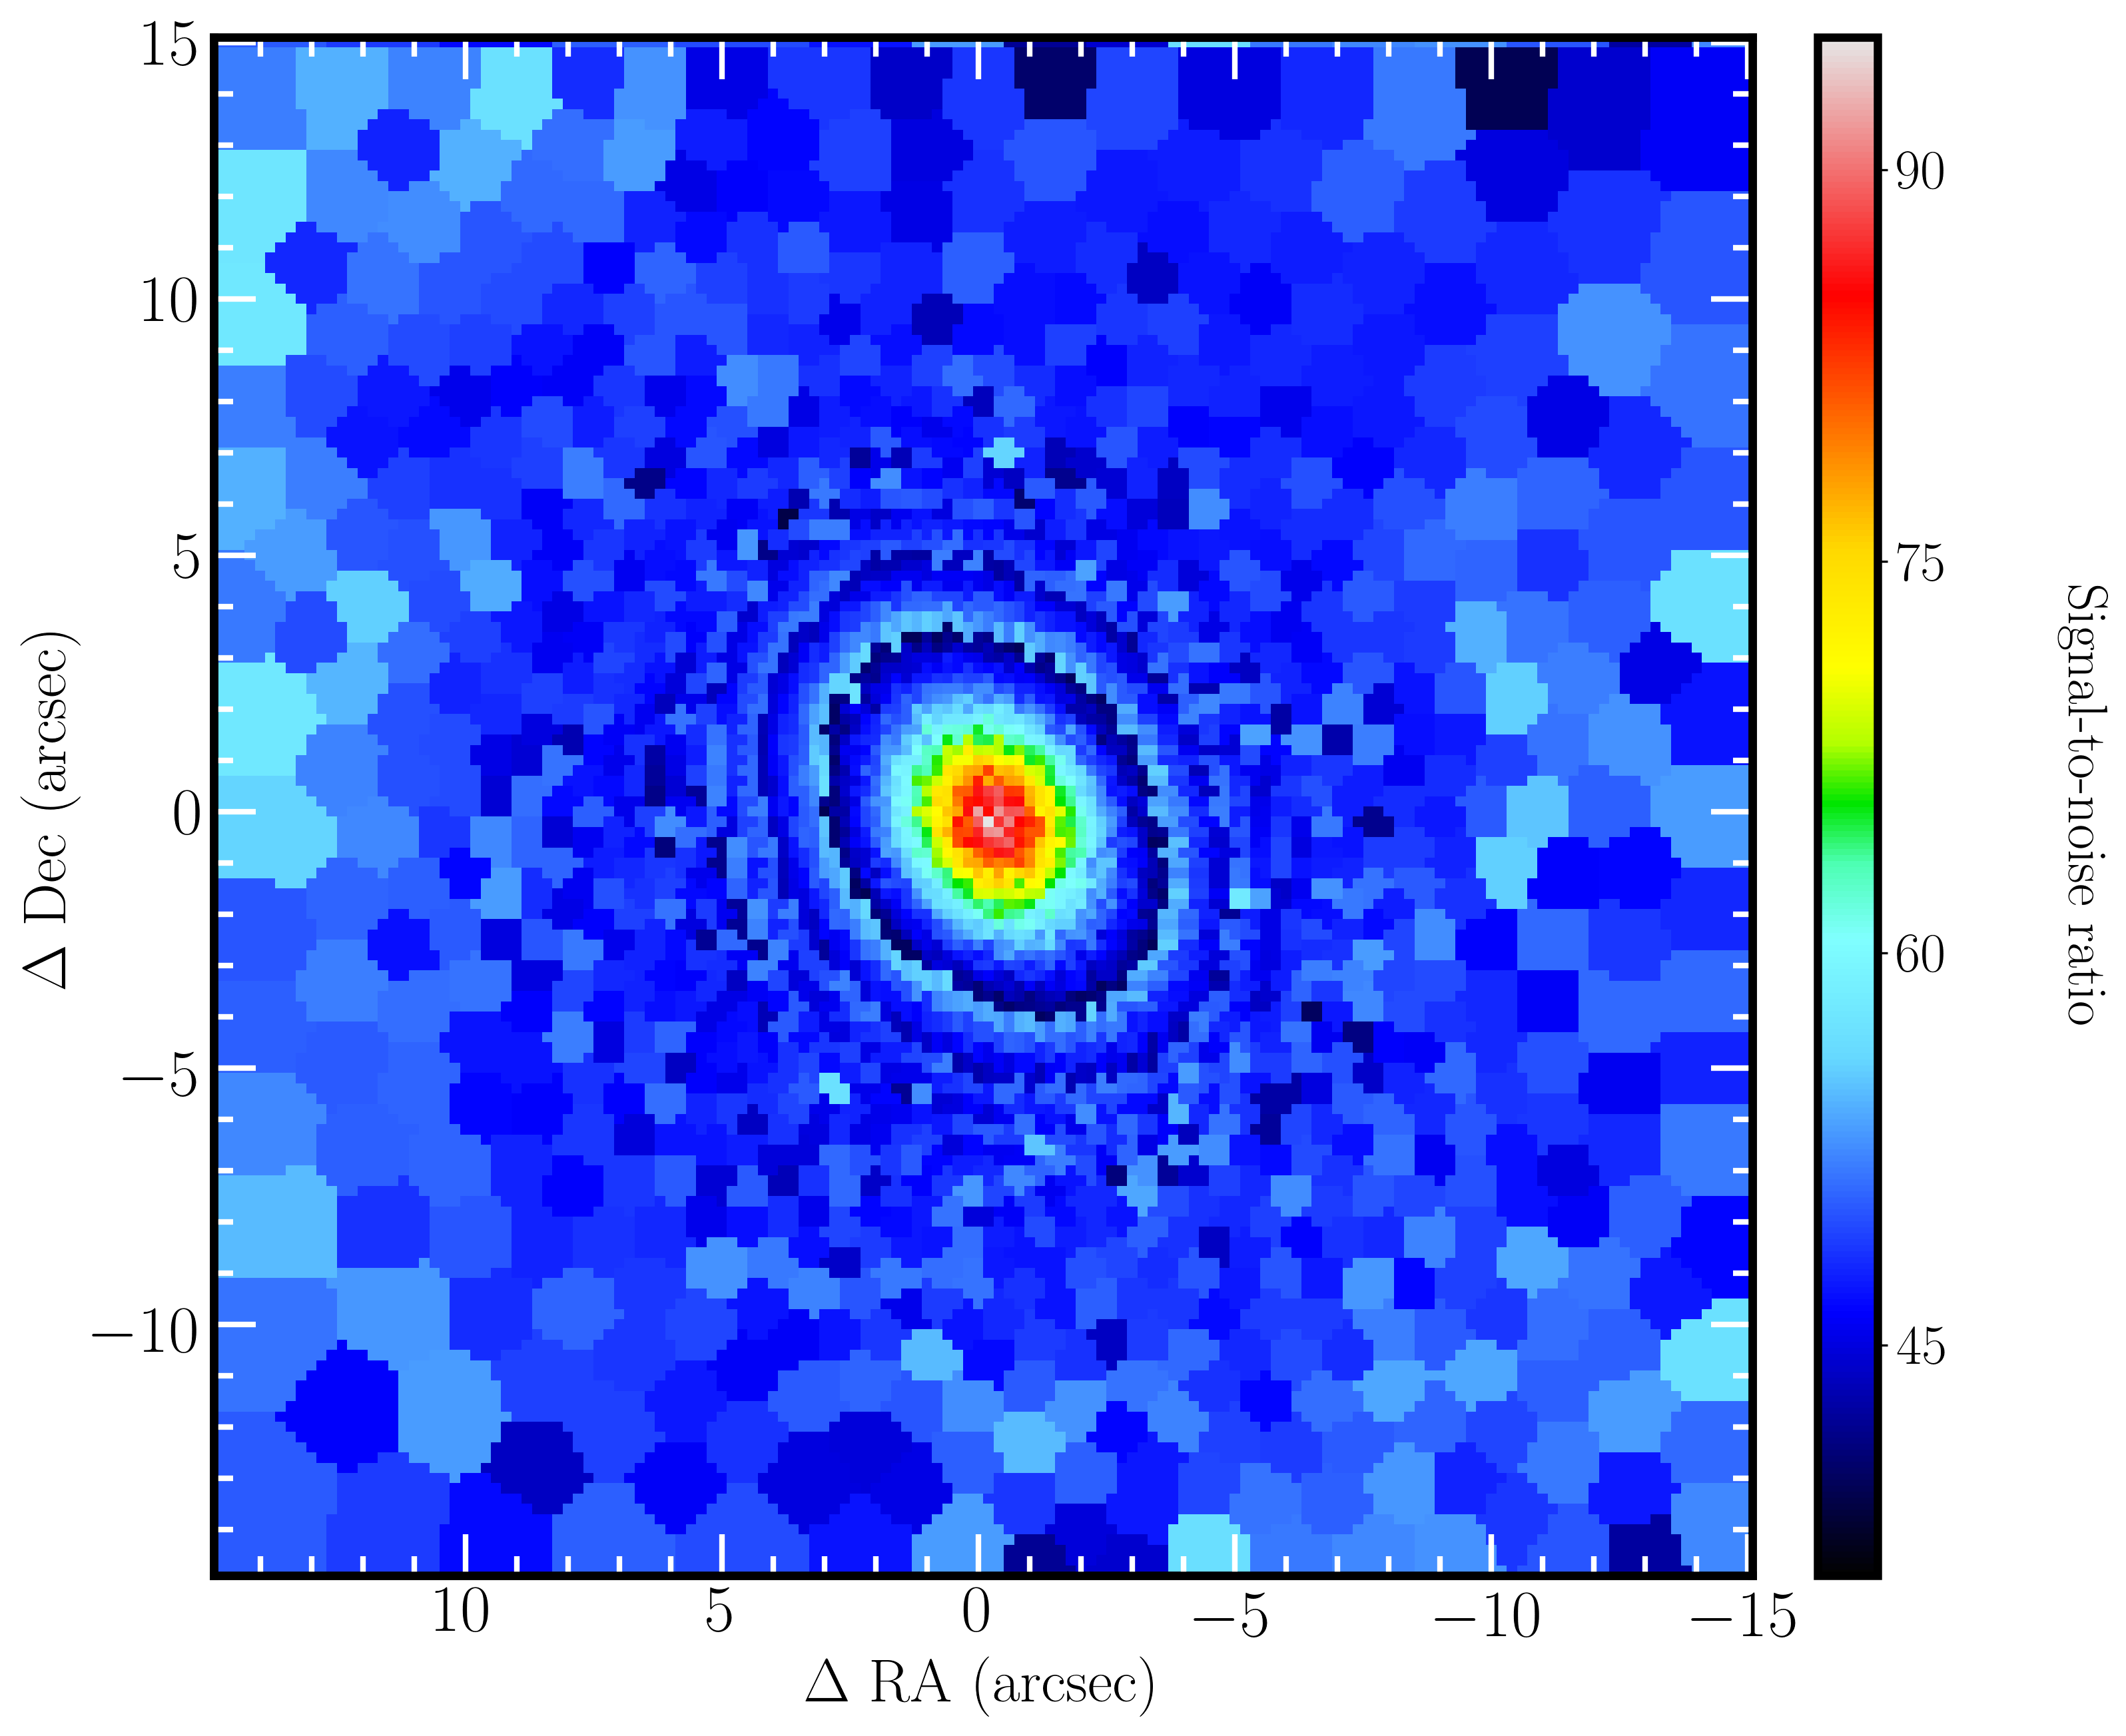
\includegraphics[width=.6\textwidth]{chapter2/egSNR.png}
			\caption[Example signal-to-noise map]{Example signal-to-noise ratio (S/N) map, from the MUSE observations of IC 1459.}
			\label{fig:egSNR}
		\end{figure}

	\subsection{Stellar Kinematics}
		\label{subsec:StellarFit}
		For our analysis, we make use of the penalized-fitting (\textsc{pPXF}) routine\footnote{\url{http://www-astro.physics.ox.ac.uk/~mxc/software/}} of \citet{Cappellari2004} and \citet{Cappellari2016a}. This routine finds the best-fitting stellar kinematics of each bin by minimizing the reduced chi-square ($\chi^2_\text{red}$) of a model spectrum built from a linear combination of empirical stellar templates, convolved with a Gaussian LOSVD (here parametrised by the mean velocity, $v$, and velocity dispersion, $\sigma$). Gaussian templates are also used to independently fit emission lines from the interstellar medium (ISM), with their own LOSVDs. Throughout our analysis, we fit all emission lines as a single component independently from the stars, and thus they have individual fluxes (except for fixed flux ratios within forbidden line doublets) but the same kinematics. \textsc{pPXF} requires an initial guess for the LOSVD of each component and we use here the redshift of the galaxy and $\sigma = 200\,\mathrm{km\,s^{-1}}$ for both components (stars and gas). Finally, Lagrange polynomials are used to make additive and/or multiplicative corrections to the continuum level of the fit. A potential sky line at 5199\,\AA\ in the Earth's frame of reference is masked in all fits.

		It was noted that for NGC 1316, the NaD absorption feature (which as generally attributed to absorption from the ISM and is thus affected by the kinematics of the ISM) was significantly effecting the quality of the stellar best-fitting spectrum. For this reason, the wavelength range of NGC 1316 spectra was limited to $<5800 \, \AA$ whilst fitting for the stellar spectra only.

		To improve the speed of our analysis, we first collapse each datacube spatially to produce a global spectrum of the galaxy, by summing across both spatial dimensions at each wavelength. The entire MILES stellar library \citep{Sanchez-Blazquez2006, Falcon-Barroso2011a} is then used to provide templates for the \textsc{pPXF} fit. We mask $600\,\mathrm{km\,s^{-1}}$--wide regions around potential emission lines (see Table \ref{tab:EmissionLine}), and use a fourth order Lagrange polynomial for an additive continuum correction. Here we use the redshift values from Simbad \citep{Wenger2000} as our initial velocity guesses. For our 14 datacubes (10 VIMOS and 4 MUSE datacubes), these fits use an average of 23 templates (with non-zero weights) out of 985. The other templates are discarded for all future analyses of a given datacube. This drastically improves the runtime of \textsc{pPXF} without affecting the quality of the fits.

		Next we implement a routine to find more optimal initial guesses of the mean velocity and velocity dispersion for each galaxy, to be used when fitting in divided bins, by means of iterative fits to the global spectrum. For each galaxy, the initial fit is set up in the same way as in the previous step, but only using the templates with non-zero weights. For each fit, the best-fitting mean velocity and velocity dispersion of the previous fit are used as the initial \textsc{pPXF} guesses, thus iteratively improving the initial guesses with each subsequent fit. The final mean velocity of a given galaxy, is used as its precise spectroscopic redshift and is given in Table \ref{tab:sample}. 

		% After the first three repetitions, the velocity was used to calculate the precise redshift of the galaxy: these are the redshift values quoted in \ref{tab:sample}. After this, small random perturbations to the iterative initial estimates are applied to ensure that the routine converges on a global minimum chi-squared, rather than a local one. 100 repetitions are run, with the mean velocities and velocity dispersions recorded and used as the initial estimates for all subsequent fits in that datacube. 

		Beyond this point, each bin is analysed independently. Each one is processed through \textsc{pPXF} using only the MILES templates with non-zero weights identified above, using the redshift and velocity dispersion estimates from the last step as initial guesses. Again, regions around potential emission lines are masked, and a fourth order polynomial additive continuum correction is used. The residuals between the best-fitting spectrum and the input spectrum are smoothed in wavelength using a weighted, moving average. This is then summed in quadrature with the noise spectrum (as propagated through the data reduction pipeline) to produce a combined `residual noise' spectrum. A Monte--Carlo (MC) estimate of the uncertainties, with 1000 repetitions is used, whereby in each iteration (after the first), random noise is added to the best-fitting model from the first run, distributed with a Gaussian profile of width equal to the residual noise. The standard deviation of the best-fitting parameters from these 1000 iterations are then adopted as the best-fitting uncertainties.

		% For accurate estimates of the uncertainties on these best-fitting values, a Monte--Carlo, with 1000 repetitions is used. In each iteration (after the first), random noise, distributed with a Gaussian profile and an amplitude comparable to the noise propagated through the data reduction pipeline, is added to the best-fitting spectrum from the first run. The standard distribution of the fitted parameters from each iteration is used as the quoted uncertainty.


	\subsection{Emission-line Kinematics}
		\label{subsec:EmissionFit}
		Deriving the distribution and kinematics of the emission lines is achieved in a manner similar to that of deriving the stellar kinematics. However, to minimize template mismatch, whereby emission lines are erroneously fitted to the edges of badly modelled and thus subtracted absorption features, we follow the method set out in \citet{Sarzi2005}. This is a three-step process, applied to each bin:
		\begin{enumerate}
			\item The region around each emission line's rest-frame wavelength is masked, and the stellar spectrum is fitted, ignoring the masked regions.
			\item The kinematics of the stellar component (i.e.\ all stellar templates) is fixed to that found in step 1. The region around the [\ion{O}{iii}] doublet is then unmasked and fitted with two (one for each doublet component) additional (and positive) Gaussians with a single free amplitude, mean velocity and velocity dispersion. The ratio of the amplitudes is fixed to 0.35.
			\item All potential emission lines are unmasked and fit with additional Gaussians, but with their kinematics fixed to that of [\ion{O}{iii}] derived in Step 2. Only the amplitudes of the Gaussians (i.e.\ the amplitude of the emission lines) therefore fit. 
		\end{enumerate}
		All the steps above are repeated with the aforementioned MC method to estimates the uncertainties, and include a tenth order multiplicative Lagrange polynomial to account for poorly modelled continuum emission. The ratio of the amplitudes of the constituent emission lines within a doublet is fixed for some forbidden lines (see Table \ref{tab:EmissionLine}).

		For each fitted emission line $i$, the ratio of the amplitude of the fitted line to the median residual noise across the line, $(A/N)_i$, is used to estimate the reliability of the detection threshold. As in \citet{Sarzi2005}, a fit to the [\ion{O}{iii}] doublet only is considered a detection if $(A/N)_{[\text{\ion{O}{iii}}]} \ge 4$. For all other lines except [\ion{N}{i}], a fit to the line is only considered a detection if [\ion{O}{iii}] is detected in the same bin and $(A/N)_i \ge 3$. For a fit to the [\ion{N}{i}] doublet, we require a detection of both [\ion{O}{iii}] and H$\beta$ and $(A/N)_{[\text{\ion{N}{i}}]} \ge 4$. The emission lines considered are listed in Table \ref{tab:EmissionLine}, along with their rest wavelengths and that of any doublet counterparts (for so-called forbidden lines). 

	 	\begin{table}
	 		\centering
	 	\begin{threeparttable}
	 		\caption{Emission lines considered in the \textsc{pPXF} fits. Every emission line given below, within the wavelength range of a given datacube was included in the analysis, thus VIMOS datacubes are fitted with H$\gamma$, H$\beta$, \brackets{\ion{O}{iii}} and \brackets{\ion{N}{i}} lines and doublets, while MUSE datacubes are fitted with H$\beta$, \brackets{\ion{O}{iii}}, \brackets{\ion{N}{i}}, \brackets{\ion{O}{i}}, \brackets{N}{ii}, H$\alpha$ and \brackets{\ion{S}{ii}} lines and doublets.}
	 		\label{tab:EmissionLine}
	 		\begin{tabular}{l c c c}
	 		\hline
	 		\hline
	 		Emission Line & Rest-frame & Doublet rest-frame & Amplitude ratio \\
	 		 & wavelength & wavelength & \\
	 		 & (\AA) & (\AA) \\
	 		\hline
	 		% \bracket{\ion{O}{ii}} 	& 3726.03 & 3728.82 & Free \\
	 		% H$\delta$ 	& 4101.76 & -- & -- \\
	 		H$\gamma$ 	& 4340.47 & -- & -- \\
	 		H$\beta$ 		& 4861.33 & -- & -- \\
	 		\bracket{\ion{O}{iii}}	& 4958.92 & 5006.84 & 0.35 \\
	 		\bracket{\ion{N}{i}} 	& 5199.36 & 5201.86 & 0.65 \\
	 		\bracket{\ion{O}{i}} 	& 6300.30 & 6363.67 & 0.33 \\
	 		\bracket{\ion{N}{ii}} 	& 6548.03 & 6583.41 & 0.34 \\
	 		H$\alpha$ 	& 6562.30 & -- & -- \\
	 		\bracket{\ion{S}{ii}} 	& 6716.47 & 6730.85 & Free \\
	 		\hline
	 		\hline
	 		\end{tabular}
	 		\begin{tablenotes}
	 		\note Col\,1: Emission line name. Col\,2: Emission line rest-frame wavelength. Col\,3: Doublet rest-frame wavelength for forbidden lines. Col\,4: The fixed ratio of the amplitudes of the lines within a doublet. `Free' indicates the amplitudes of both doublet constituents are fit independently of each other. 
	 		\end{tablenotes}
	 	\end{threeparttable}
	 	\end{table}




	 \subsection{Stellar Populations}
	 	\label{subsec:PopFit}
	 	To investigate the stellar populations of our sample galaxies we assume that a given spectrum (a global, spatially-integrated spectrum or the spectrum of a single bin) is well approximated by a single stellar population (SSP), i.e.\ that this spectrum is well represented by a collection of stars all born at the same time, in the same environment (i.e.\ with a unique combination of age, metallicity and $\alpha$-element over/under-abundance). 

	 	There are two methods to find the best-fitting SSP: full spectral fitting using synthetic spectra with different properties, and comparison of empirical or modelled line strengths to observed absorption line strengths. The former has the advantage of utilizing more information, fitting fine structure features in the spectrum and easily finding complex stellar populations. It does, however, rely on highly accurate synthetic spectra for each combination of stellar population properties considered. Also, for massive ETGs, fine spectral feature are lost because of the smoothing caused by the high velocity dispersions. The latter has the advantage of only considering the parts of the spectrum that are highly sensitive to the stellar population. It can also more easily be based on empirical observations of stars in the solar neighbourhood, and is thus less model dependent.
	 	% Interpolation between well-populated regions of the parameter space of the stellar population properties can be used to minimize the errors in sparse regions of the parameter space. 
	 	We also found that full spectral fitting almost always converged to an extreme corner of the parameter space, presumably because the model spectra are not accurate enough or our data still contains instrumental artefacts. For these reasons, we adopted the absorption line strength approach.

	 	\subsubsection{Absorption Line Strengths}
	 		\label{subsubsec:Absorption}
	 		Absorption line strength indices are defined as equivalent widths. Each index consists of 3 bandpasses: one blue and one red continuum bandpass on either side of a central bandpass containing the absorption feature of interest. A pseudo-continuum $F_\mathrm{C}(\lambda)$ is defined as the straight line between the two continuum bandpasses, assigning the median flux of each bandpass to its central wavelength. The index $I$ is then measured as the equivalent width of the spectrum $F_\mathrm{I}(\lambda)$ within the central bandpass (sampling from wavelength $\lambda_1$ to $\lambda_2$), with respect to the pseudo-continuum. For the so-called atomic indices, measured in \AA, this yields
	 		\begin{align}
	 			I_\text{\AA} \equiv \, & \int^{\lambda_2}_{\lambda_1} \! \left[1 - \frac{F_\mathrm{I}(\lambda)}{F_\mathrm{C}(\lambda)}\right] \, \mathrm{d}\lambda \, , \\
	 		\intertext{while for molecular indices, measured in magnitude, this yields}
	 			I_\text{mag} \equiv \, & -2.5 \log\left[\frac{1}{\lambda_2 - \lambda_1} \int^{\lambda_2}_{\lambda_1} \! \frac{F_\mathrm{I}(\lambda)}{F_\mathrm{C}(\lambda)} \, \mathrm{d}\lambda\right] \, .
	 		\end{align}
	 		The indices used for this project, along with their defining rest-frame bandpasses, are taken from \citet{Trager1998} and are listed in Table \ref{tab:abIndex}. All spectra are appropriately shifted to account for their systematic stellar velocity (redshift). 

		 	\begin{table}
				\centering
			\begin{threeparttable}
				\caption{Line index bandpass definitions. All absorption indices where the entirety of all bandpasses within the rest-frame wavelength range of a given datacube are measured, thus G4300, Fe4383, Ca4455, Fe4531, H$\beta$ and Fe5015 indices are measured for all VIMOS datacubes, while Mg\,b is measured for most VIMOS datacubes (the red continuum band is redshifted out of the wavelength range of NGC 612 and PKS 718-34). H$\beta$, Fe5015, Mg\,b, Fe5270, Fe5335, Fe5406, Fe5709, Fe5782, NaD, TiO1 and TiO2 are measured for all MUSE datacubes.}
				\label{tab:abIndex}
				\begin{tabular}{l c c c}
					\hline
					\hline
					Index 	& Blue continuum & Index band & Red continuum \\
					 & (\AA) & (\AA) & (\AA) \\ 
					\hline 
					G4300 	& 4266.375\,--\,4282.625 & 4281.375\,--\,4316.375 & 4318.875\,--\,4335.125 \\
					Fe4383 	& 4359.125\,--\,4370.375 & 4369.125\,--\,4420.375 & 4442.875\,--\,4455.375 \\
					Ca4455 	& 4445.875\,--\,4454.625 & 4452.125\,--\,4474.625 & 4477.125\,--\,4492.125 \\
					Fe4531 	& 4504.250\,--\,4514.250 & 4514.250\,--\,4559.250 & 4560.500\,--\,4579.250 \\
					H$\beta$ & 4827.875\,--\,4847.875 & 4847.875\,--\,4876.625 & 4876.625\,--\,4891.625 \\
					Fe5015 	& 4946.500\,--\,4977.750 & 4977.750\,--\,5054.000 & 5054.000\,--\,5065.250 \\
					Mg\,b 	& 5142.625\,--\,5161.375 & 5160.125\,--\,5192.625 & 5191.375\,--\,5206.375 \\
					Fe5270 	& 5233.150\,--\,5248.150 & 5245.650\,--\,5285.650 & 5285.650\,--\,5318.150 \\
					Fe5335 	& 5304.625\,--\,5315.875 & 5312.125\,--\,5352.125 & 5353.375\,--\,5363.375 \\
					Fe5406 	& 5376.250\,--\,5387.500 & 5387.500\,--\,5415.000 & 5415.000\,--\,5425.000 \\
					Fe5709 	& 5672.875\,--\,5696.625 & 5696.625\,--\,5720.375 & 5722.875\,--\,5736.625 \\
					Fe5782 	& 5765.375\,--\,5775.375 & 5776.625\,--\,5796.625 & 5797.875\,--\,5811.625 \\
					NaD 	& 5860.625\,--\,5875.625 & 5876.875\,--\,5909.375 & 5922.125\,--\,5948.125 \\
					TiO1 	& 5816.625\,--\,5849.125 & 5936.625\,--\,5994.125 & 6038.625\,--\,6103.625 \\
					TiO2 	& 6066.625\,--\,6141.625 & 6189.625\,--\,6272.125 & 6372.625\,--\,6415.125 \\
					\hline
					\hline
				\end{tabular}
				\begin{tablenotes}
				\footnotesize
				\note All index definitions are from \citet{Trager1998}. All bandpasses are defined in the rest frame and as such all spectra must be appropriately shifted to account for the redshift of the stars. 
				\end{tablenotes}
			\end{threeparttable}
			\end{table}

			Much of the literature provides absorption line strength measurements in the Lick/Cassegrain Image Dissector Scanner spectrograph system (hereafter Lick/IDS system; \citealt{Faber1985, Worthey1994}), but this has several disadvantages. Firstly, the Lick/IDS system is based on non-flux-calibrated spectra from the IDS spectrograph on the Shane telescope (Lick Observatory), that has a relatively low and wavelength-dependent spectral resolution. When using the Lick/IDS system with other instruments, it is thus necessary to calibrate the observations by performing empirical corrections aiming to compensate for the uncalibrated continua of the Lick/IDS data. This requires observations of standard stars using the same instrumental set-up as the main observations. Since this was not requested as part of the VIMOS observing strategy and standard star observations are thus unavailable, we are unable to transform our measurements to the Lick/IDS system. An additional/new proposal is not possible either, as VIMOS has been substantially upgraded in the intervening time. Given the low spectral resolution and poor data quality on which the Lick/IDS system is based, we believe in any case that the community should be making a concerted effort to use alternative systems. We therefore choose to use the line index system (LIS) of \citet{Vazdekis2010}. LIS is based on flux-calibrated measurements at several spectral resolutions (5.0, 8.4 and 14.0\,\AA\ FWHM). \citet{Vazdekis2010} also provide empirical cubic functions to transform Lick/IDS literature measurements to LIS\footnote{\url{http://www.iac.es/proyecto/miles/pages/line-index-system-lis/transformations.php}}.

			Because of the models we use for stellar population fitting (see Section \ref{subsubsec:StellarPop}), we actually measure the absorption line indices at a slightly degraded spectral resolution of 2.5\,\AA. For comparisons to the literature (Section \ref{subsec:absorption}), we also measure the absorption line indices at 8.4\,\AA\ resolution. 

			Since our aim is to find the best-fitting stellar population model, it is important to first remove the contribution of the ISM to the spectra. This involves fitting for and subtracting the emission lines detected (as described in Section \ref{subsec:EmissionFit}). 

			We must also correct for the effect of the different velocity dispersions of the stellar populations, that varyingly spread absorption features such that differing fractions of the absorption are outside of the central bandpasses. To do this, we simply create a best-fitting spectrum (as in the previous step) that is not convolved with the best-fitting LOSVD. Note that for NGC 1316, for indices with a wavelength longer than 5800\,\AA\, we use the extrapolated best-fitting pPXF fit. A given index, $I$, is then measured for both this `unconvolved' spectrum ($I^\text{unc}$) and the convolved best-fitting spectrum ($I^\text{conv}$), and the ratio of these two indices is used as a multiplicative correction factor for the index measured ($I^\text{obs}$), such that the corrected index ($I^\text{corr}$) is given by
			\begin{equation}
				I^\text{corr} \equiv \frac{I^\text{unc}}{I^\text{conv}} I^\text{obs} \, .
			\end{equation}
			These corrected indices are those reported and discussed in the sections below and in Section \ref{subsec:absorption}.


		\subsubsection{Stellar Population Models}
			\label{subsubsec:StellarPop}
			The final step of the data analysis pipeline is to find the best-fitting SSP model of a given spectrum. Sets of SSP models consist of a grid of models characterised by stellar properties such as age ($t$), metallicity ([Fe/H]) and alpha-element enhancement ([$\alpha$/Fe]). Here, we first provide a generic overview of the process of generating synthetic stellar population models, and then detail the specific of the models adopted. 

			Synthetic SSPs are created using the following components:
			\begin{itemize}
				\item the paths of stars of a given mass and metallicity as they travel across the Hertzsprung--Russell diagram (HRD) by ageing. These are known as stellar evolutionary tracks and are generally empirical.
				\item the function $\Phi(M)$, representing the number of stars formed $N(M)$ per mass interval $\mathrm{d}M$, i.e.\ $\Phi(M) \equiv \frac{\mathrm{d}N(M)}{\mathrm{d}M}$. This is the initial mass function (IMF).
				\item an empirical library of stellar spectra, to be able to assign a spectrum to each position on the HRD. 
			\end{itemize}
			The desired output of expected line strengths for a three-dimensional grid of varying age, metallicity and $\alpha$-enhancement can be computed in one of two ways: (i) by producing full synthetic spectra from the stellar evolution models sampled very finely as a function of the tree stellar parameters of interest or (ii) by finding a `fitting function' for each index, that analytically relates the index measured from an empirical library to the three stellar parameters of interest. The former is dependent on a good understanding of the physics of stellar atmospheres and is known to suffer from incomplete line lists and continuum uncertainties \citep{Thomas2004}. This would have been the appropriate method for producing synthetic spectra for full spectral fitting had we chosen that method for investigating the stellar populations of our sample galaxies (see Section \ref{subsec:PopFit}). The latter, and more popular, method allows for interpolation between well-populated regions of stellar parameter space in order to increase the accuracy of the models in stellar parameter space that are only sparsely sampled by an empirical stellar library \citep{Thomas2010}. 

			\begin{figure}
				\centering
				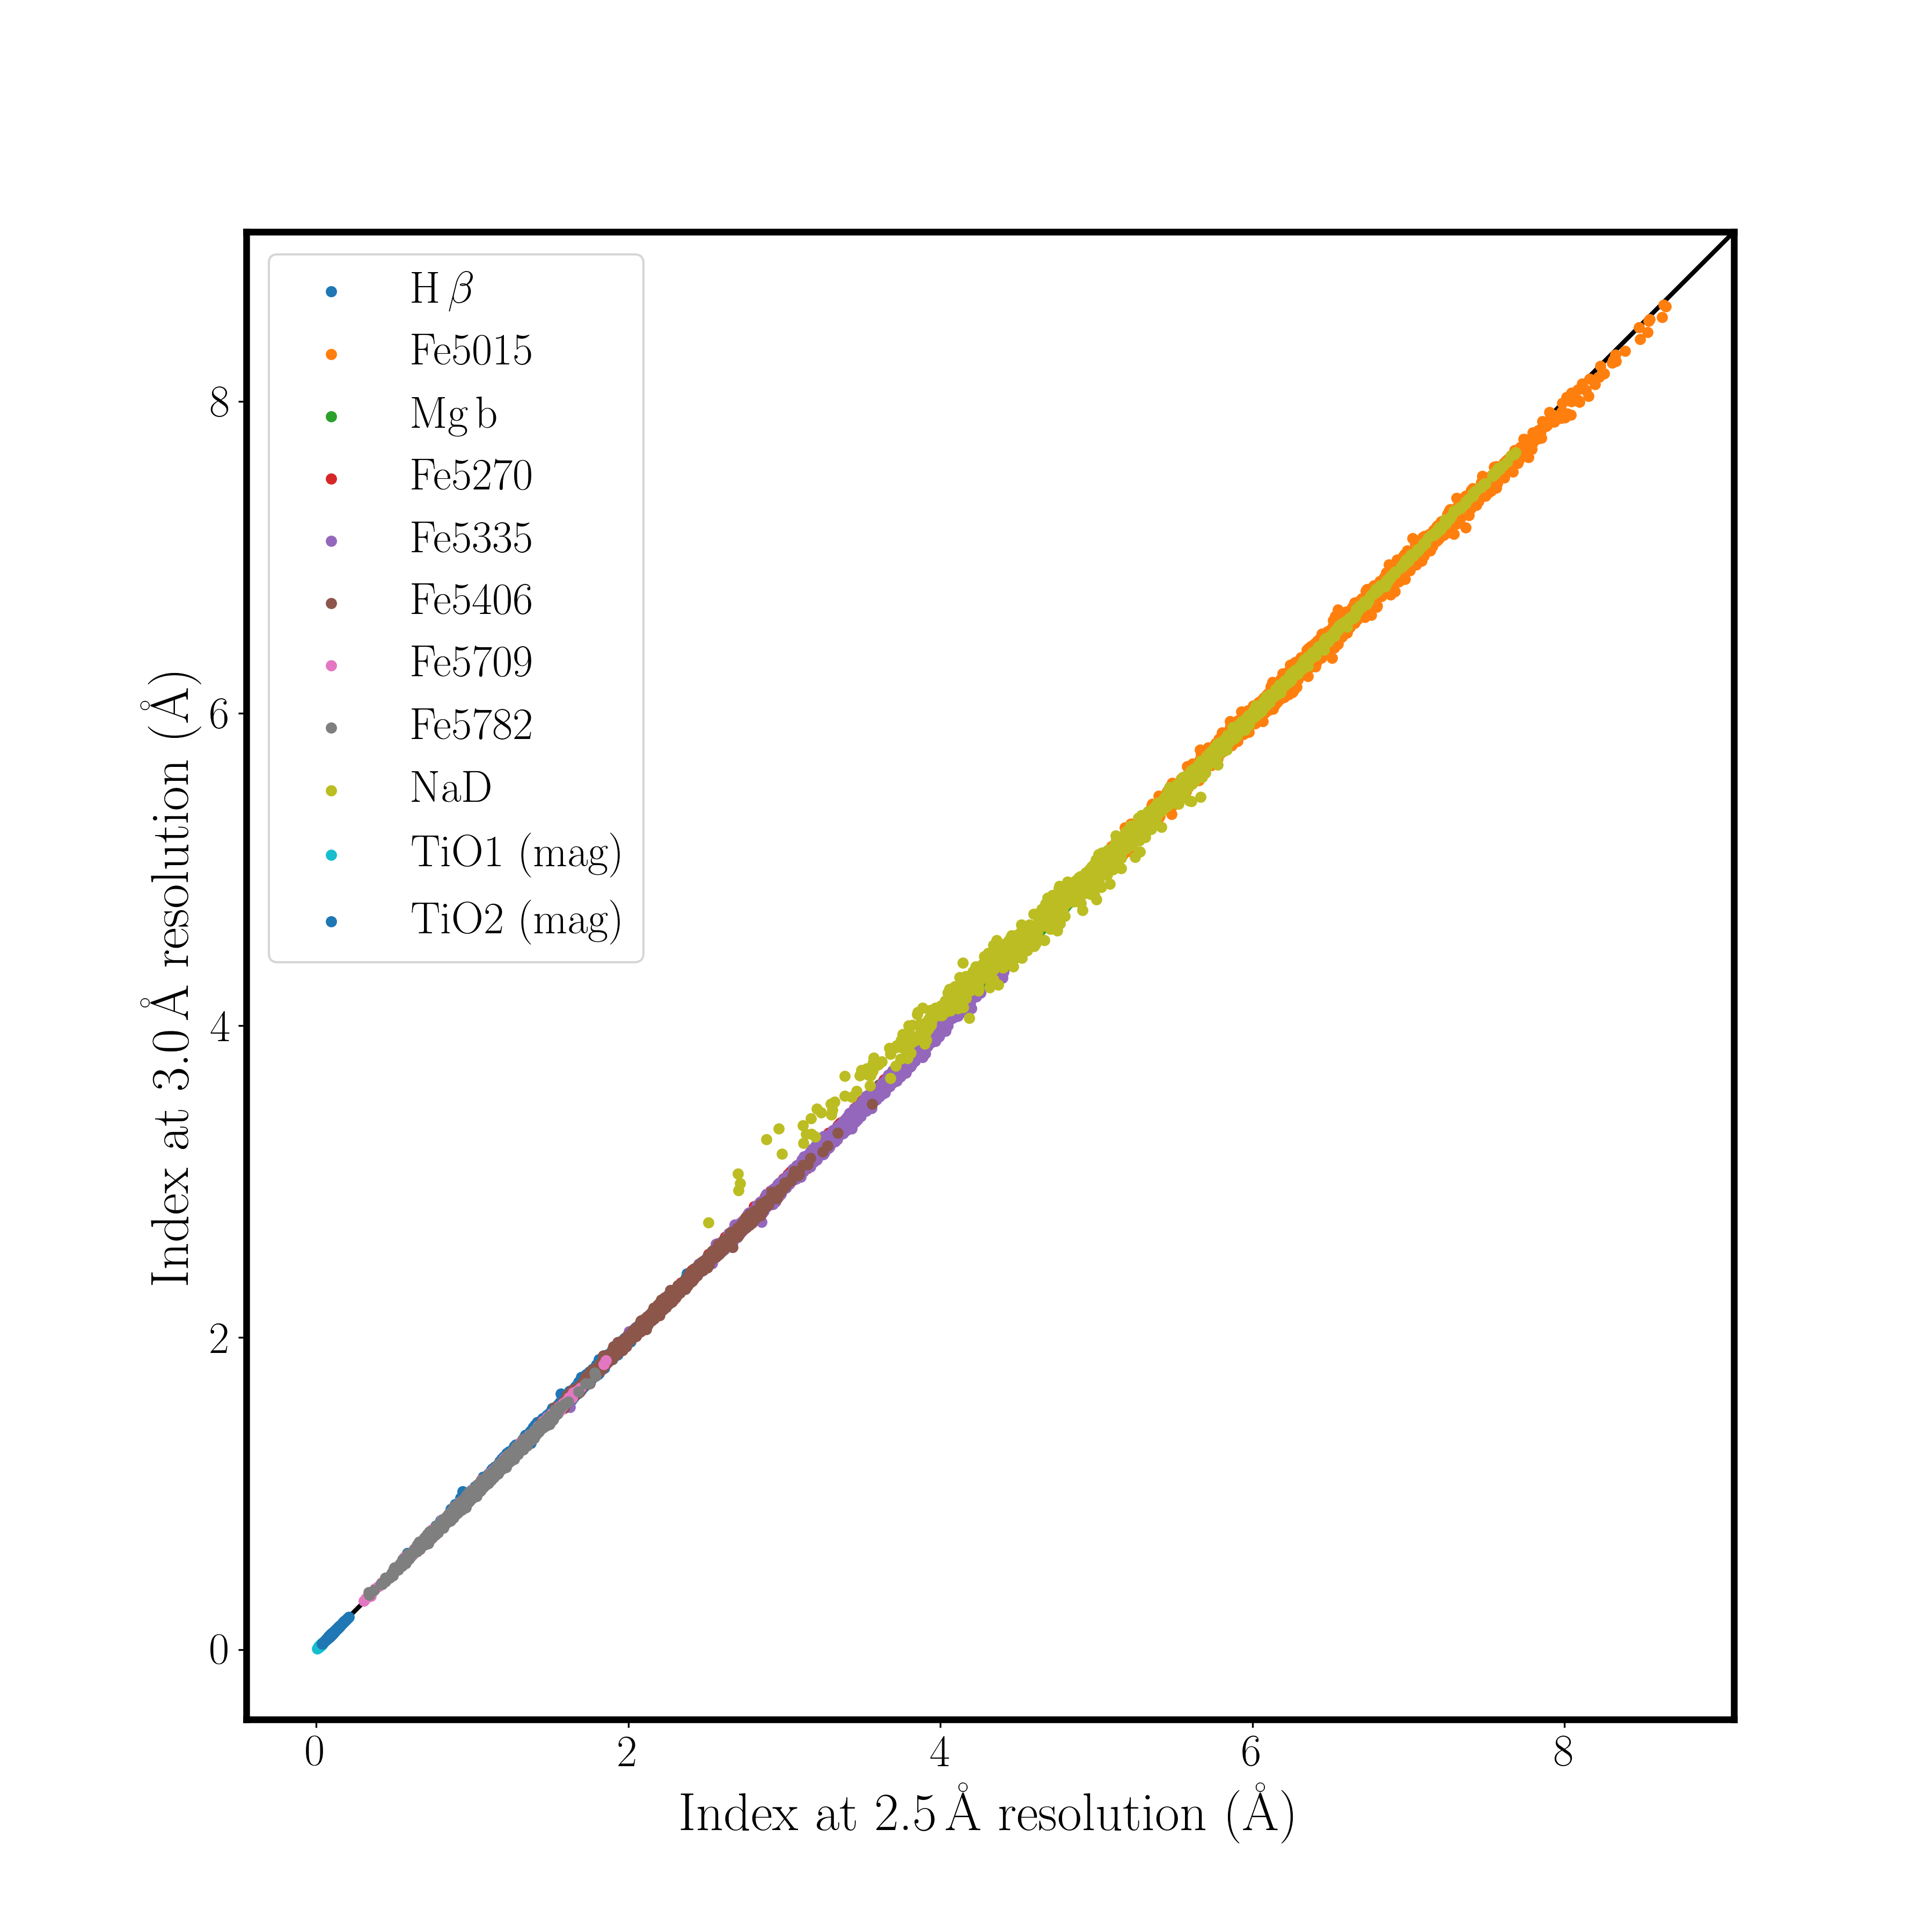
\includegraphics[width=.7\textwidth]{chapter2/compare_resolutions.png}
				\caption[Resolution effects on absorption line index strengths]{Resolution effect on absorption line strength measurements. Absorption line strength indices at 2.5\AA\ and 3.0\AA\ spectral resolution are compared, showing that the effect of a slightly lower spectral resolution is negligible. The dotted lines mark a difference of $\pm1$\% between the measurements at each resolution.}
				\label{fig:res}
			\end{figure}

			ETGs often have very different fractional abundances of the various metals than those of the nearby stars that we are able to observe (all of which have near solar abundances). As such, the empirical stellar libraries used to calibrate the models fall short of the required coverage of parameter space. Most methods somehow attempt to extrapolate their results to non-solar abundances, and in a similar way to the fitting functions described above, `index response functions' can be constructed. These attempt to calibrate the effects of the varying abundances of individual elements, and comparison must then be made to completely theoretical spectra.

			Here we use the SSP models of \citeauthor{Thomas2010} (\citeyear{Thomas2010}; hereafter TMJ), as they are based on flux-calibrated spectra and therefore do not require calibration to the Lick/IDS system. These models assume a \citet{Salpeter1955} IMF ($\Phi(M) \propto M^{-2.35}$) and are based on the evolutionary population synthesis code of \citet{Maraston1998}. The models use the stellar evolutionary tracks of \citet{Cassisi1997} for metallicities $[Z/H] < -0.33$ and of \citet{Girardi2000} for $[Z/H] \ge -0.33$, the MILES stellar spectral library of \citet{Sanchez-Blazquez2006a} and \citet{Falcon-Barroso2011a}, the fitting functions of \citet{Johansson2010} and the index response functions of \citet{Korn2005}. The MILES library and thus the models have spectral resolution of 2.5\,\AA. This is better then the resolution of the reduced VIMOS data (3\,\AA), but we show in Fig.\,\ref{fig:res} that this has a negligible effect. Indeed, comparing the absorption line strengths measured at 2.5\,\AA\ and 3\,\AA\ for the MUSE datasets shows that the worst affected index is Fe5782 with a mean difference of only 1\% between the indices measured at 3\,\AA\ and 2.5\,\AA\ resolution. All other indices show a difference of only a few tenths of a percent. 

			The response functions of \citet{Korn2005} extend the work of \citet{Tripicco1995}, who investigated the response functions of the original 21 Lick indices when the individual element abundance fractions are varied for a 5 Gyr old SSP at solar metallicity. The new functions include varying metallicities as well as individual element fractions, and are calculated for all 25 Lick indices. The effect of age on these response functions was tested by computing them for 1 Gyr models and comparing them to the 5 Gyr models of \citet{Tripicco1995}. \citet{Korn2005} found a 1\% difference for two indices (G4300 and Fe4383) and significantly smaller differences for all other indices, thus concluding that age does not significantly affect the response functions.

			Finally, individual element abundances are combined to calculate the alpha-element enhancement parameter [$\alpha$/Fe]. This is done following \citet{Trager2000}, who grouped the elements into three categories: 
			\begin{itemize}
				\item enhanced elements, including C, N, O, Na, Mg, Si, Ca and Ti (i.e.\ $\alpha$ and light elements); 
				\item depressed elements, including Cr and Fe (i.e.\ iron peak elements); and
				\item fixed elements (all other elements). 
			\end{itemize}
			The fixed-element group elements are held at solar abundances, while the enhanced-(depressed-)element group elements are scaled up (down) by the same factor. 

			The TMJ models return absorption line strength indices for a 3 dimensional grid ($t$, $[Z/H]$, [$\alpha$/Fe]) with $t$ = 0.1, 0.2, 0.4, 0.6, 0.8, 1, 2, 3, 4, 5, 6, 7, 8, 9, 10, 11, 12, 13, 14 and 15 Gyr; $[Z/H]$ = -2.25, -1.35, -0.33, 0.0, 0.35 and 0.67; and [$\alpha$/Fe] = -0.3, 0.0, 0.3 and 0.5.

			TMJ showed that their models produce good fits to globular cluster measurements of \citet{Puzia2002} and \citet{Schiavon2005} and the galaxy measurements of the SAURON team by \citet{Kuntschner2010}. \citet{Conroy2010} suggest that the stellar evolutionary tracks of \citet{Girardi2000} used for the high-metallicity models do not fit the globular clusters well, but TMJ point out that this can be explained by an anomaly in the Balmer lines that is not present in the SAURON data analysis. TMJ therefore suggest that this is an issue with the globular cluster measurements themselves. 

			% Following the method of \citet{McDermid2006}, we first linearly interpolate the TMJ models to a three-dimensional grid with sides of length 40 in age, metallicity and $\alpha$-enhancement. The metallicity and $\alpha$-enhancement axes are linearly sampled, while the age axis is logarithmically sampled. 

			Markov chain Monte--Carlo (MCMC) fitting is useful as it allows for the efficient exploration of parameter space by avoiding regions with low probabilities (high $\chi^2_\text{red}$). A large number of `walkers' are placed at an initial position (the hypothesis). In each iteration, each walker moves a random distance in a random direction. For a given walker, if the probability is higher at its new location it accepts the move, otherwise it is rejected and the walker remains in its initial position. In this thesis we choose to use \textsc{emcee}, a \textsc{python} MCMC fitting package \citep{Foreman-Mackey2013}. \textsc{emcee} is an ensemble MCMC sampler, meaning that the steps taken by each walker are influenced by the position of all the other walkers. This allows for a quicker convergence on the most-likely result. After first interpolating the 3-dimensional grid of TMJ SSP models using \textsc{LinearNDInterpolator} (a \textsc{python} package provided in \textsc{scipy}; \citealt{Barber1996}), we use the MCMC method to find the most-likely SSP model, by comparing the absorption line strength indices measured (with the method described above in Section \ref{subsubsec:Absorption}) to those of the interpolated grid models. \textsc{emcee} is an affine-invariant ensemble MCMC sampler meaning that we can take the standard deviation of the positions of the walkers in the MCMC code as the uncertainty on the most-likely stellar population.

			In Section \ref{sec:pop} we will use the results from this pipeline to compare the absorption line strength indices and the stellar populations of our Southern Sample radio galaxies to those of radio-quiet ETGs.
